% Page number location defaults to bottom-center
% Use \documentclass[pagenumtop]{wsu-thesis} to get page numbers at top-right
%email JMcDonald1@wsu.edu for latex help
\documentclass{wsu-thesis}

% Some packages are already added by the wsu-thesis class
% Check the wsu-thesis.cls file if you have any issues
\usepackage{graphicx}
\graphicspath{{\figuredir/}} %\figuredir defined below
\usepackage{tensor}
\usepackage{siunitx}
\usepackage{float}
\usepackage[numbers]{natbib}
\usepackage{xcolor} % Remove after notes are no longer needed
\usepackage{longtable}
\usepackage{array}


% Front matter information
% Title needs to be inverted pyramid shape, may need manual breaks using \\
\title{MEASUREMENTS AND MODELING OF ARCTIC ATMOSPHERIC\\PROCESSES DURING THE NORWEGIAN YOUNG SEA ICE\\FIELD CAMPAIGN}
%Use your full name as it appears on your transcripts}
\author{Sarah Yvette Murphy}
%Indicate if it is a Dissertation (doctoral) or Thesis (master's)
\thesistype{Dissertation}
%Fill out the full degree name
\degree{Doctor of Philosophy in Engineering Science}
%Official name of department, school, program, or college that grants your degree
\department{Voiland School of Engineering and Architecture, Department of Civil and Environmental Engineering}
%Fill out the month your degree is awarded, rather than the month you defend.
\submitmonth{April}
\submityear{2023}

% Useful definitions
\newcommand{\phd}{Ph.D.}
\newcommand{\chapterdir}{./chapters}
\newcommand{\frontmatterdir}{./front-matter}
\newcommand{\appendixdir}{./appendices}
\newcommand{\referencedir}{./references}
\newcommand{\figuredir}{./figures}

\begin{document}
% Create title page and blank second page
% Use \maketitle* if you wish to remove copyright info
\maketitle

% Create signature page with requisite text
\begin{signaturepage}
  % \signature creates line for signature with committee member's full
  % name and degree.  Make sure you check with each committee member so that you have this correct before you print your  cotton pages.  Comment out or delete extra lines or [Co-chair]
  \signature{Von P. Walden}{\phd}[Chair]
  \signature{Stephen Hudson}{\phd}
  \signature{Brian Lamb}{\phd}
  \signature{Heping Liu}{\phd}
  \signature{Hailong Wang}{\phd}
\end{signaturepage}

% Acknowledgement page is optional, remove if not needed
% The title can be changed with \begin{acknowledgements}[New Title]
\begin{acknowledgements}
  %% MEASUREMENTS
% N-ICE
The N-ICE field campaign was supported by the Norwegian Polar Institute's Centre for Ice, Climate and Ecosystems (ICE) through the N-ICE project, and the Research Council of Norway through the STASIS project (221961/F20). 

% SCGSR Fellowship
The modeling using the idealized version of WRF and the flux equation research (Chapters 5 and 6) were partially supported by the U.S. Department of Energy, Office of Science, Office of Workforce Development for Teachers and Scientists, Office of Science Graduate Student Research (SCGSR) program. The SCGSR program is administered by the Oak Ridge Institute for Science and Education (ORISE) for the DOE. ORISE is managed by ORAU under contract number DE‐SC0014664. All opinions expressed in this document are the author’s and do not necessarily reflect the policies and views of DOE, ORAU, or ORISE.

% Cheyenne
NCAR's Cheyenne supercomputer was used for all Polar WRF simulations except for the idealized WRF simulations. We would like to acknowledge high-performance computing support from Cheyenne (doi:10.5065/D6RX99HX) provided by NCAR's Computational and Information Systems Laboratory, sponsored by the National Science Foundation.

%% PYTHON
The author would like to thank the Python community for the open-source data science tools, including wrf-python \citep{wrfpython}, xarray \citep{xarray}, and matplotlib \citep{matplotlib}. All were used extensively throughout this dissertation. 

%% PEOPLE
Chapter 3 was made possible with help from Dr. Keith Hines (Polar Meteorology Group, Byrd Polar and Climate Research Center at The Ohio State University), who provided useful insight to help get the Polar WRF model running on the Washington State University supercomputer. Dr. Hines also assisted in some early decisions regarding the setup of Polar WRF, including insight into input data sets and formatting of WRF configuration files.

Dr. Xiang-Yu Li (Pacific Northwest National Laboratory) helped with the setup of the idealized WRF model and troubleshooting some model issues. The author would like to thank him for the helpful conversations and for taking the time to help translate WRF error files.

Dr. Lana Cohen provided research advice from the perspective of someone who was on the ship at N-ICE and helped clarify some of the caveats of the measurement data. Conversations with her have helped with the details of Chapters 2 and 3. 

This research for this dissertation was supported by the National Science Foundation grants PLR-1304657, PLR-1314248, NNA-1801764, OPP-2110341.
\end{acknowledgements}

% Abstract arguments are degree YOU are earning and committee chair(s) names
\begin{abstract}{\phd}{Von P. Walden}
  The Arctic is warming more quickly than other regions due to Arctic amplification, resulting in modifications to the surface energy budget. The Norwegian Young Sea Ice (N-ICE) field campaign took place in January through June 2015, monitoring key components of the surface energy budget. This was the first field campaign to take observations of the surface energy budget in the winter since the Surface Heat Budget of the Arctic (SHEBA) field campaign in 1997 through 1998. These observations are valuable not only due to the amount of time that has passed since the SHEBA field experiment but also because N-ICE took place on younger, thinner sea ice, and in a different part of the Arctic. This study uses data from the N-ICE experiment to recommend improvements to the Polar Weather Research and Forecasting (WRF) model. The goals of this study are: 1) compare atmospheric measurements to models, 2) investigate model cloud microphysics and boundary layer parameterizations within WRF, 3) determine what cloud properties were observed during N-ICE, 4) investigate the effects of turbulent fluxes and clouds on young sea ice, and 5) make recommendations for improving the Polar WRF model. The Polar WRF model results show that there were issues in calculating both the turbulent and radiative fluxes over first-year sea ice. The cloud conditions during N-ICE varied, and mixed-phase clouds (mixture of water and ice) were seen throughout the entire experiment. The model, however, did not accurately simulate the radiative impacts of these clouds. To determine if the calculations of sensible and latent heat flux can be accurately estimated given the correct cloud conditions, a study was conducted comparing turbulent fluxes from the Maximum Energy Production method and the bulk flux algorithm (based on Monin-Obukhov theory and the technique used to estimate fluxes within WRF). Sensible heat flux was accurately estimated, but all equations overestimated the amount of latent heat flux. When compared to an idealized (offline) version of the WRF model using the measured radiative fluxes as input, the WRF model estimates the turbulent fluxes well, indicating that the model is using an appropriate version of the flux equations and that most of the error within the model can be attributed to the cloud properties.
\end{abstract}

% Remove List of Figures or List of Tables if not needed
\tableofcontents
\listoffigures
\listoftables

% Main chapters
\begin{mainchapters}
  \chapter{About the Polar Regions}
\vspace{1 cm}
\begin{spacing}{1} \begin{quote} 
\noindent \emph{Stronger warming in the Arctic than in the global average has already been observed and its causes are well understood. It is very likely that the warming in the Arctic will be more pronounced than on global average over the 21st century (high confidence).} \end{quote}
\hspace{6 cm} - IPCC Sixth Assessment Report, August 2021  
\end{spacing}
\vspace{1 cm}


\section{The Arctic and Climate Change}
The largest impacts of climate change are those seen in the Arctic. Over the past several decades, Arctic temperatures have increased more than the global average by 2.5 \citep{tjernstrom:2014a}, due largely to Arctic amplification \citep{rantanen:2022}. This is a series of mechanisms in which the polar regions undergo positive feedback loops which can change the energy balance at the surface. Arctic amplification includes the ice-albedo effect, which amplifies temperature increases due to greenhouse gas emissions by melting sea ice. As sea ice melts, the albedo of the surface decreases, resulting in more solar energy absorption. As the surface absorbs more solar energy, it warms, increasing Arctic air temperatures, which melts additional sea ice. This is a key example of a positive feedback loop \citep{ipcc_techsum}. A second example of Arctic amplification occurs when permafrost thaws, releasing stored methane into the atmosphere. This increase in atmospheric methane increases the greenhouse effect, further increasing permafrost melt. To fully understand Arctic climate change, it is crucial for scientists to study this region and the physical processes that contribute to Arctic amplification.

Arctic climate change heavily impacts marine life, indigenous people, and coastal ecosystems \citep{ipcc_techsum}. However, these local impacts are not the only thing to be concerned about. Changes in Arctic sea ice can cause irreversible changes in the atmospheric and oceanic circulation. Many CMIP5 models indicate that within the next few years,  the Earth may experience ice-free conditions during the summer \citep{stroeve:2018}.

Sea ice has been declining at an increasing rate throughout the last decade due to increased melt seasons replacing multi-year sea ice with thin, first-year sea ice \citep{meier:2014}. \citet{wunderling:2020} found that 55 $\%$ of the additional warming in the Arctic was a result of ice-albedo feedback. The rest is attributed to a change in lapse rate and cloud properties resulting in increased surface heating. These changes have resulted in an ice loss of approximately 3.4 $\%$ per decade. Multi-year sea ice has decreased from 59 $\%$ of the ice pack to 28 $\%$ in 2018 and continues to decrease \citep{stroeve:2018}. As a result, the fraction of first-year ice has increased.  Because of this, there is a need to fully understand atmosphere-ocean interactions over first-year ice. 

\section{Surface Energy Budget}
The surface energy budget can influence ice growth or melt. A study done using SHEBA observations over sea ice show that the ice and snow thickness has a significant impact on the surface temperature and, as a result, the surface energy budget, due to the changes in heat transfer through the snow and ice \citep{hines:2015}. Additionally, the surface energy budget is often misrepresented in models due to an underestimation of cloud cover, resulting in downward longwave radiation biases \citep{inoue:2008}. Eq. \ref{eq:qnetintro} and \ref{eq:r} show the surface energy budget and net radiation equations.

\begin{equation}\label{eq:qnetintrointro}
Q_{net} = (Q_{sw_down} - Q_{sw_up}) + (Q_{lw_down} - Q_{lw_up})
\end{equation}

\begin{equation}\label{eq:r}
R = Q_{net} + H_{s} + H_{l}
\end{equation}

Where $Q_{sw}$ and $Q_{lw}$ are the shortwave and longwave radiative fluxes respectively with the arrow denoting upward vs downward, R is the residual flux, including heat transfer through the ice and heat storage, and $H_{s}$ and $H_{l}$ are the sensible and latent heat fluxes. While net radiative flux can easily be measured or estimated given temperature profiles and cloud cover, values such as the sensible and latent heat fluxes are not as straightforward to estimate. Models often have skill in one value but have large compensating errors in other values. These values are heavily influenced by both the clouds and the near-surface boundary layer structure \citep{tjernstrom:2005}.

\subsection{Clouds: Longwave and Shortwave Radiation}

Due to complexities in cloud feedback and the underlying surface, there are a variety of ways models handle cloud formation and properties. Properties such as proximity to melt ponds/open water, the shape of the snow crystals, and snow depth, can all influence how clouds modify surface radiation. Arctic atmospheric models, while key to understanding cloud processes, are not perfect, and still have trouble quantifying these processes. 

A key feedback mechanism in the arctic regions is the cloud radiation feedback, which, unlike other Arctic amplification feedback, can be either positive or negative depending on influences such as the cloud properties and sun angle. This process is nonlinear and can be either positive or negative. This process applies all over the globe, but due to the high surface albedo and lack of atmospheric moisture, it has the potential to influence the surface radiation budget more in the Arctic. Further research is necessary to quantify the exact influence. When clouds are lower in the atmosphere or are more optically thick they emit more longwave radiation. However, a cooler cloud, one higher in the atmosphere or thin, would radiate less longwave radiation, but still more than under clear-sky conditions. This is an example of how clouds can warm the surface. On the other hand, clouds can cool the surface as a result of their shortwave impact. The higher the cloud albedo (optically thicker the cloud), the more shortwave radiation is reflected away, not reaching the surface, and not being included in the surface energy budget. \citet{intrieri:2002} studied the radiative influence of clouds at SHEBA and found that, for the SHEBA location, the net cloud effect was to warm the surface through most of the year, with only a short two-week period in the middle of the summer, when the location was getting the most direct solar radiation when clouds had a cooling influence on the surface by reflecting shortwave radiation away from the surface. 

Cloud radiative forcing (CRF) is often used to quantify the impacts of clouds on surface radiation. This is defined in Eq. \ref{eq:crf}, but can be conceptually understood as the difference between the surface radiation in the absence of clouds ($Q_{clear sky}$) and the actual radiation ($Q_{actual}$). A large positive (negative) cloud radiative forcing indicates surface warming (cooling) due to cloud radiative influence. 

\begin{equation}\label{eq:crf}
CRF = Q_{actual} - Q_{clear sky}
\end{equation}

\subsection{Sensible and Sensible Heat Flux}

The near-surface planetary boundary layer (PBL) is often strongly stable in the Arctic due to significant surface radiative cooling compared to the ambient temperature. This is due to a combination of the cold surface and the small-to-nonexistent diurnal cycle. Additionally, the latent heat of phase change in the surface during the melt season also acts to cool the air closest to the surface, creating a stable boundary layer. Models, however, often have a difficult time simulating these strongly stable conditions, and either forms a PBL not stable enough or too stable for actual conditions.  Regional models are generally better than this and can be used to improve larger-scale models, but there is still a need for further model improvement. The fluxes influencing the boundary layer are strongly influenced by the cloud conditions, and a model with inaccurate clouds will likely also have inaccurate boundary layer conditions and fluxes \citep{tjernstrom:2005}. 

\section{Arctic Measurements}

One of the first major experiments studying meteorology and ice dynamics took place between 1975 and 1976. This experiment, The Arctic Ice Dynamics Joint Experiment (AIDJEX), was led by the University of Washington and consisted of four ice camps with surrounding buoys. Taking measurements over sea ice is both dangerous and difficult as deployment and maintenance is nearly impossible without the aid of a ship. Other ways of taking in-situ measurements include floating buoys, but the measurement capabilities of buoys are limited by the lack of available onboard power. Research vessels are utilized for their ability to provide power, transportation, and housing for scientists while observing the Arctic.

A series of ship-borne experiments took place between 1991 and 2001: the International Arctic Ocean Experiment (AOE) (1991), AOE-96 (1996) \citep{tjernstrom:2004}, the Surface Heat Budget of the Arctic  Experiment (SHEBA) (October 1997 - October 1998) \citep{uttal:2002}, and AOE (2001). The earlier two AOE focused on atmospheric aerosols and did not include vertical profiles of atmospheric structure or ice characteristics.  The 2001 AOE experiment focused more extensively on meteorological variables \citep{tjernstrom:2004}. SHEBA had a larger array of meteorological instruments, observing both the cloud properties and the surface energy budget over sea ice for an entire year \citep{uttal:2002}. Before the Norwegian Young Sea Ice Campaign (N-ICE2015) took place in January of 2015, SHEBA (described in the next subsection) was the most recent experiment to observe these atmospheric properties. 

\subsection{SHEBA}

SHEBA took place onboard a Canadian Coast Guard ice breaker, the Des Groseillers, in the Beaufort Sea north of Alaska from 1997 to 1998 \citep{uttal:2002, shupe:2004}. The ship sailed north from Alaska and was intentionally frozen into the sea ice and allowed to drift with the ice \citep{uttal:2002}. Helicopter flights also surveyed the area to document the ice conditions surrounding the ship and a tethered balloon was utilized to observe the boundary layer conditions. The primary goals of this experiment were to observe the changes occurring in the surface energy budget over sea ice as the polar regions undergo global warming with the hope that these observations can give both context to the poorly understood mechanisms occurring under these never-before-observed conditions and to provide observations to validate and improve general circulation models in the Arctic \citep{uttal:2002}. Particular focus was on ocean-ice-atmosphere feedbacks, such as the ice-albedo and cloud-radiation feedback during the entire annual cycle. 

The ice pack SHEBA was frozen into varied in thickness from 1.8 $m$ (October) to 2.6 $m$ (June) and was classified as multiyear sea ice, indicating this ice pack had not completely melted the previous summer. Snowpack was also observed on the ice throughout the experiment, reaching a maximum depth in June, when 30 $cm$ of snow fell but melted quickly in the following days \citep{uttal:2002}. Multi-year sea ice is becoming less prominent on the polar regions, and first-year sea ice is beginning to dominate the Arctic. This shift away from the conditions seen at SHEBA and toward thinner, first-year sea ice is a motivation for N-ICE2015, which took observed conditions over young sea ice \citep{graham:2017}. 

During the start of SHEBA, the western Arctic had an anomalously large amount of multi-year ice. In addition, the autumn upper ocean had a lower salinity and warmer temperature than expected, indicating a larger ocean heat flux than was typical of the area during the summer resulting in the larger melt due to the reduction in sea ice cover the previous year. Comparing SHEBA data to estimates from other field experiments showed that during transition seasons (September, October, November, March, and April), SHEBA had larger incoming longwave radiation by 2 to 45 $Wm^{-2}$ than other studies. This could be caused by either an increase in the number of warm air masses over SHEBA or an increase in cloud cover \citep{persson:2002}. SHEBA was an important field experiment that filled many gaps in our understanding of cloud and radiation processes. One of the most important findings from SHEBA was that, even at temperatures well below freezing, mixed-phase clouds occurred often. 



\subsubsection{Remaining Questions from SHEBA}



\section{Arctic Modeling}
The Polar Meteorology Group at the Ohio State University Byrd Polar Research Center developed a series of enhancements to the Weather Research and Forecasting Model (WRF). Additions to the model are always being added, but at the time of writing, modifications have been made to the surface energy budget over ice, an updating sea-ice mask, and changes to microphysics. Testing has been completed using datasets from Alaska, Antarctica, and Greenland. The only studies over sea ice that have been done used data collected from SHEBA and, now, N-ICE. 

\section{Dissertation Outline and Attributions}
Chapter two will go into detail about the measurements made at N-ICE, including meteorological conditions and cloud radiative forcing. Analysis for this chapter was completed by Sarah, with LiDAR processing and section x.x completed by Dr. Robert Stillwell. Dr. Von Walden and Dr. Stephen Hudson were advisors on this research. 

Using these measurements, chapter 3 compares the latent and sensible heat flux observed at N-ICE to fluxes calculated using the Maximum Entropy Method and a Bulk Flux algorithm. These methods of calculating fluxes depend on exchange coefficients and surface stability, which is also thoroughly explored in chapter 3. Chapter 4 looks into how a popular weather model simulates the conditions seen at N-ICE and how changing parameters built into the model can influence the resulting fluxes. All research, coding, analysis, and writing was completed by Sarah with advice from Dr. Hailong Wang and Dr. Von Walden. Part of this research was done in collaboration with Pacific Northwest National Lab as part of the Department of Energy's Office of Science Graduate Student Research Program (DOE SCGSR).

The equations used in the model are broken down in Chapter 5, comparing them to the methods of calculating flux in Chapter 3. This chapter uses the measurements described in chapter 2, the equations explored in chapter 3, and the modeling schemes detailed in chapter 4 to answer the question "Can we improve how models simulate fluxes over first-year sea ice?" This chapter also includes further pathways this research could take.

In addition to the work presented in the following chapters, I completed data processing of the flux data. Appendix B documents the process of determining the sensitivity of EddyPro's results to gaps in the input datasets and if artificially filling these gaps is the most accurate way to represent this missing data. This data was used in a dataset \citep{nicefluxes:2017} and in a publication \citep{walden:2017} on which I am the 4th author.



  \chapter{The Norwegian Young Sea Ice Field Campaign}
\vspace{1 cm}
\begin{spacing}{1} \begin{quote} 
\noindent \emph{Earth system observations are an essential driver of progress in our understanding of climate change. Overall, capabilities to observe the physical climate system have continued to improve and expand. Improvements are particularly evident in ocean observing networks and remote-sensing systems.} \end{quote}
\hspace{6 cm} - IPCC Sixth Assessment Report, August 2021  
\end{spacing}
\doublespacing
\section{Introduction}
The Norwegian Young Sea Ice field campaign (N-ICE2015 or N-ICE) was a 6-month field campaign conducted from January to July 2015, observing both atmospheric properties and sea ice dynamics. During this period, a Norwegian research icebreaker vessel, the RV Lance, was frozen into the sea ice north of Svalbard and allowed to move with the ice floes. The ship tracks can be seen in \ref{fig:nice}. Three times during the expedition the ice surrounding the ship broke up and the ship needed to be repositioned into the sea ice. The time it took for the ship to reposition can be seen as gaps in the data from 21 February, through 24 February, 15 March through 24 April, and again from 5 June through 7 June. The period in March and April corresponds with a trip back to Svalbard for resupply, explaining the long duration of the data gap. The dates of each ice floe are listed in table \ref{tab:floedates}. 

\begin{figure}[b!]
    \centering
    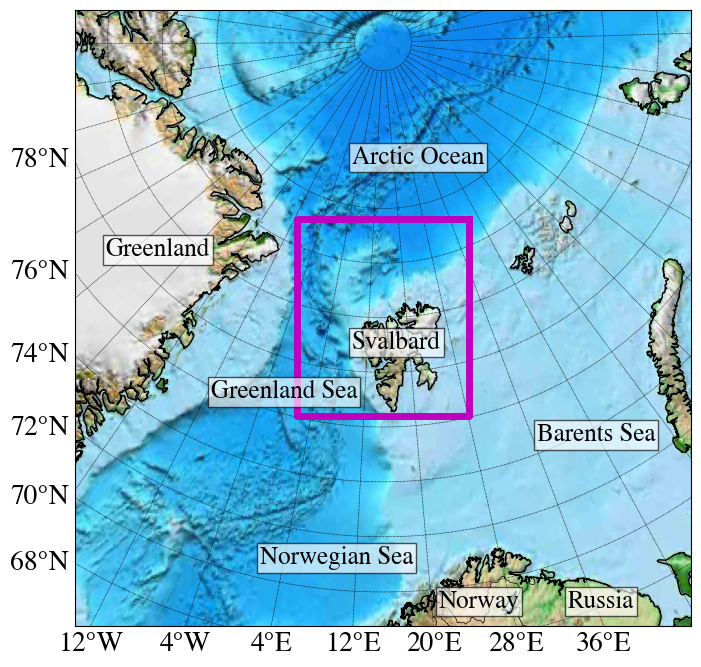
\includegraphics[width=0.5\linewidth]{figures/chapter2/ship_zoom_out.png}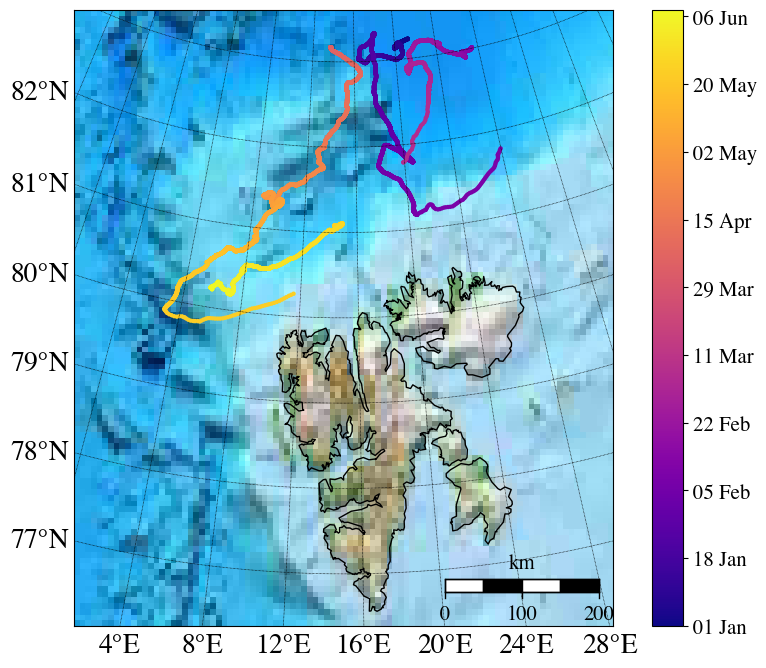
\includegraphics[width=0.55\linewidth]{figures/chapter2/ship_zoom_in.png}
    \caption[N-ICE location.]{The location of the N-ICE field expedition. The right map shows a detailed view of the area indicated by the purple box on the left map. Ship location is plotted on the right figure and is colored by date.}
    \label{fig:nice}
\end{figure}

\begin{table}[t!]
\centering
\footnotesize
\doublespacing
{
\begin{tabular}{| c | c | c | c | c  |}
 \hline
\rowcolor[HTML]{F3F3F3}  &  &  & \multicolumn{2}{ c |}{\textbf{Ice Edge Proximity}} \\
\rowcolor[HTML]{F3F3F3} 
\multirow{-2}{*}{\textbf{Floe}} & \multirow{-2}{*}{\textbf{Start Date}} & \multirow{-2}{*}{\textbf{End Date}} & \textbf{Min Distance} & \textbf{Max Distance} \\
  \hline
 1 & 15 January 2015 & 21 February 2015 & 50 km & 175 km\\
 2 & 24 February 2015 & 19 March 2015 & 200 km & 325 km\\ 
 3 & 18 April 2015 & 5 June 2015 & 225 km & 40 km \\
 4 & 7 June 2015 & 21 June 2015 & 85 km & 10 km \\
  \hline
\end{tabular}}
\caption[N-ICE floe dates and ice edge proximity.]{Floe does and approximate proximity to ice edge for the N-ICE field campaign.}
\label{tab:floedates}
\end{table}

This region is characterized by thin, first-year (or ``young") sea ice, as opposed to the thick, multi-year sea ice observed during SHEBA \citep{cohen:2017}. As a result, the N-ICE measurements are representative of the new regime that the polar regions are moving toward as the climate warms. This expedition is of particular interest from a modeling perspective due to the magnitude of the temperature and pressure change during and after winter storm periods. This research cruise is the first to take measurements of the clouds and atmosphere since SHEBA in 1997 and 1998. These concurrent measurements of the energy budget and cloud properties (fraction, height, microphysical, and temperature) can give important insight into climate processes and radiative transfer \citep{persson:2002, schweiger:2004}. 

\citet{shupe:2004} observed mixed-phase clouds during SHEBA were consistent in temperature, liquid water path, and ice water content with previous studies over similar sea ice. NICE2015 observed more extreme storm periods than those seen at SHEBA, bringing wind speed, pressure, and temperature changes of previously unobserved magnitudes. In general, the winter during N-ICE was characterized by several significant storm periods \citep{cohen:2017}. These storms were associated with significant changes in surface temperature and humidity conditions, as well as changes in cloud properties. Springtime conditions during N-ICE were more normal with a gradual increase in surface temperatures and fairly constant thick cloud cover \citep{cohen:2017}.

Throughout much of N-ICE, strong temperature inversions were observed over the surface, similar to what was seen at SHEBA \citep{kayser:2017}. While these strong inversions are not unique to N-ICE2015, they are often underrepresented in Polar WRF simulations \citep{hines:2015}. 
\newline 
\noindent The primary objectives of N-ICE are:
\begin{enumerate}
    \item To quantify the change in atmosphere-ice-ocean interactions as the atmosphere shifts from primarily multi-year sea ice to thin, first-year sea ice \citep{granskog:2018, granskog:2015}. 
    \item To observe how changes in sea ice impact the marine ecosystem and their response \citep{granskog:2015}.
    \item To provide key observations to tune and validate models \citep{granskog:2018, granskog:2015}.
\end{enumerate}

 The overall conditions during the field campaign are described by \citet{cohen:2017}, \citet{kayser:2017}, and \citet{walden:2017}. More details about the experiment and the datasets that were collected can be found in \citet{granskog:2015}. \citet{itkin:2017} describes the proximity to the sea ice edge throughout the experiment. During the majority of the experiment, the ship was stationed between 50 and 250 $km$ from the ice edge during the first 3 floes. Approximate distances to the ice edge during each floe are listed in Table \ref{tab:floedates} \citep{oikkonen:2017}.

\section{Instruments}
A variety of instruments were deployed during the N-ICE campaign that will be used in this project, including radiosondes, a MicroPulse Lidar (MPL), a meteorological tower, an Eddy Covariance (EC) system, and broadband shortwave and longwave radiometers. 

Vaisala RS92-SGP radiosondes were launched from the ice surface (Floe 1) or the ship deck (Floes 2, 3, and 4) twice daily around 1100 and 2300 UTC. The radiosondes recorded temperature, relative humidity, wind speed and direction, pressure, and geopotential height as high as 30 $km$. Data were recorded by the radiosondes every two seconds and were transmitted to the ground using a Vaisala MW31 ground station \citep{kayser:2017, cohen:2017}. More information and analysis of the radiosondes can be found in \citet{kayser:2017}.

Data from the MPL were recorded every 14 seconds up to a height of 18 $km$. The MPL records backscattered light from clouds and operates at 532 $nm$. The range resolution is 15 m, with an 18 km maximum cloud base height. Distance uncertainties are $\pm$ 2$\%$ due to timing uncertainties within the instrument. This instrument is more sensitive to water particles than ice, so some cloud types may be biased toward higher percentages of water than ice within the cloud. The MPL is easily attenuated by optically thick clouds. In some instances when a low water cloud is detected, it is possible that more cloud layers exist above this layer that cannot be measured by the MPL. 

A meteorological tower was deployed on the ice 300 to 400 $m$ away from the ship. This tower was set up within a few days of anchoring to each new floe and recorded relative humidity and temperature (Vaisala HMP155), pressure (RM Young 61302 V), and wind speed and direction (Lufft Ventus V200A-UMB) at 2, 4, and 10 $m$ heights. All measurements were collected by a Campbell Scientific CR30000 data logger at 1-second resolution. Periods of missing tower data were reconstructed using temperature and wind information from the ship (sensors mounted 22 to 24 $m$ above the surface). More information about the meteorological measurements, temperature, and wind reconstruction using the ship data, a diagram of the meteorological tower setup, and a comparison of the meteorology to SHEBA can be found in \citet{cohen:2017}.

Radiometers (Kipp and Zonen CMP22 and CGR4) were set up 1 to 1.2 $m$ above the surface near the meteorological tower to measure upward and downward components of longwave and shortwave components of radiation. Kipp and Zonen CVF4 ventilation units were used to heat and ventilate the radiometers to avoid riming and frosting of the radiometer domes. More information about the radiometers and an analysis of the surface energy budget can be found in \citet{walden:2017}.

Turbulent flux data were collected by a closed path EC flux system (Campbell CPEC200) mostly at  20 $Hz$ (but occasionally 10 $Hz$). This system contains a sonic anemometer and a closed-path, infrared gas analyzer. These instruments allow observation of the heat and moment exchanges and the water vapor and carbon dioxide mixing ratios, respectively. This system was set up next to the meteorological tower over a snow-covered surface. Further information about the EC Flux system can be found in \citet{walden:2017}.

\section{Atmospheric components of the surface energy budget over young sea ice}
\citet{walden:2017} detailed the turbulent and radiative fluxes over thin sea ice during N-ICE. This manuscript also discussed the surface and atmospheric conditions. Snow albedo was around 0.85 in the winter and between 0.72 and 0.80 in the spring and summer. Stable stability was found in the winter, followed by unstable conditions in the spring, and approximately neutral stability in the summer (once the skin temperature reached 0$^{\circ}C$). Latent and sensible heat flux values ranged between -10 to +10 $Wm^{-2}$ and -100 to +100 $Wm^{-2}$, respectively, in both the winter and spring. Shortwave radiation was not seen at the field site until March, at which time the sun rose and shortwave radiation increased until downward values reached almost 800 $Wm^{-2}$ mid-day near the end of the experiment. Downward longwave radiation ranged from 110 to 125 $Wm^{-2}$ during clear-sky times, and reached around 300 $Wm^{-2}$ under cloudy conditions. Positive values indicate flux into the surface.

Murphy's contribution to \cite{walden:2017} was to solve several problems with the flux dataset collected during the N-ICE campaign and to process the data through the EddyPro software. The most restrictive data problem was the number of data gaps throughout 30-minute data files, which was caused by a programming error in the datalogger. In some cases, the amount of missing data made the file unable to be processed. To fix this, the data were filled by taking the section of data before it (or after, in the case that the missing data was too close to the start of the dataset) and replicating it for the time period with no recorded data. To ensure that this method of data filling was acceptable, data from Barrow, Alaska was used to compare the post-processed data of a complete dataset with the post-processed results from the same dataset after (artificially added) gaps had been filled. Analysis of both the difference in sensible heat fluxes and the turbulent spectra from before and after the data filling were examined and determined the filling method appropriate for the type of gaps in the N-ICE data. Details of this gap-filling study were written as a report for a course on flux measurements. This report can be seen in Appendix B. 
  \chapter{Latent and Sensible Heat Flux Calculations over First-Year Sea Ice}


%%%    I'M NOT DONE THIS CHAPTER
%%%     PLEASE DONT EDIT THIS CHAPTER YET
%%%    THANK YOU! :) 


\\
\noindent Sarah Y. Murphy$^1$, Von P. Walden$^1$, Hailong Wang$^2$, Stephen R. Hudson$^3$\\

\\
\noindent $^1$Washington State University, Pullman, Washington, USA\\
$^2$Pacific Northwest National Laboratory, Richland, Washington, USA\\
$^3$Norwegian Polar Institute, Fram Centre, Tromsø, Norway\\

\begin{spacing}{1}

\noindent \textbf{Abstract}

 \noindent Sensible and latent heat flux values measured during the N-ICE2015 experiment calculated using LiCor’s EddyPro7 software are used as validation for methods of calculated surface fluxes over first-year sea ice. Fluxes can be calculated using equations based on the Monin-Obukhov similarity theory (bulk flux algorithm) and the more recently developed Maximum Entropy Production method. The Bulk Flux Algorithm is what is typically used in models and is currently used in many atmospheric models. There are parameters present in these equations that represent estimations of surface properties, such as stability, which can be underestimated in the polar regions when strong stability is observed near the surface. Ten different sets of stability-dependent equations for universal functions have been tested for use during the N-ICE field experiment. These universal function values are used in both the bulk flux algorithm and the Maximum Entropy method. The MEP method estimates the surface fluxes without requiring transfer coefficients and empirically defined values. This approach does not require as many measured variables as the bulk approach of calculating these fluxes, resulting in not only an increased ease of use, but also reduces error sources. Both equations have been tested with ten popular sets of equations for the surface stability functions. 
\end{spacing}

\doublespacing
\section{Introduction}

% why is SEB important
Understanding the energy budget at the sea ice surface is of particular importance as small changes in radiation can set off feedback loops that can result in significant climate implications. Reductions in sea ice have been found to amplify the impacts of global warming \cite{wunderling:2020} \cite{ipcc_techsum}. Differences in the surface features and atmospheric conditions present challenges for modeling the surface energy and water balances \cite{wang:2009}. 

\begin{equation}\label{eq:seb}
F_{s} - C = Q_{net} + H_{s} + H_{l}
\end{equation}

% what is the sensible and latent heat flux physically?
The energy budget can be seen in \ref{eq:seb}. The net radiative flux, $Q_{net}$, is the solar and terrestrial radiation, $F_{s}$ is the energy storage, and $C$ is the heat flux from the underlying ocean \cite{walden:2017}. The turbulent fluxes, $H_{s}$ and $H_{l}$, are the sensible and latent heat flux, and are the focus of this paper. Physically, the sensible heat flux represents a chance in temperature. A positive sensible heat flux represents surface warming, as the atmospheric temperatures are warmer than the ice surface. This is often the case during the winter, when advection brings warm air over the frozen surface. Negative sensible heat flux values represent the opposite, the surface is warmer than the atmosphere and is heating the overlying air. Latent heat flux is the heat associated with a phase change; positive latent heat flux is representative of condensation or freezing at the surface, and a negative indicates melting, evaporation, or sublimation.

% measuring SEB
Some components of the energy budget, such as the shortwave and longwave radiation, can be measured directly with radiometers. The sensible and latent heat flux, however, are more difficult to measure. A common approach to taking these measurements is the Eddy Covariance theory, which has been built into LiCor's EddyPro 7 \cite{epro} software for processing flux measurements. This program takes high-frequency measurements of surface fluxes, conducts calibration and filtering, then calculates the sensible and latent heat fluxes, along with $H_{2}0$, $CH_{4}$, $CO_{2}$ and other trace gasses \cite{epro_man}. However, an eddy covariance system is required to take the appropriate measurements to use the Eddy Covariance theory, and without the appropriate system, it is impossible to process the data using EddyPro. 

% field capaigns measuring the SEB
The Norwegian Young Sea Ice Field Campaign (N-ICE) in 2015 and the Surface Heat Budget of the Arctic Ocean Experiment (SHEBA) in 1998 both deployed eddy covariance systems, radiometers, and meteorological towers over sea ice in the Arctic ocean. SHEBA took place over older, multi-year sea ice, and the data collected has been processed both using Eddy Covariance theory and using other methods not requiring the eddy covariance system. N-ICE took place on young, first-year sea ice. A description of the fluxes observed by the eddy covariance system and radiometers can be found in Walden et al., \cite{walden:2017}, which describes the observed surface energy budget at N-ICE in detail. 


\section{Calculating Sensible and Latent Heat Flux}
Sensible and latent heat fluxes for N-ICE were been calculated using LiCor’s EddyPro7 software \cite{epro}. In this paper, the values estimated by EddyPro are compared to two methods of estimating sensible and latent heat flux: a bulk flux algorithm based in Monin-Obukhov similarity theory \cite{foken:2008} and the Maximum Entropy Production method (MEP) \cite{zhang:2021, wang:2014, wang:2009}. Both methods estimate flux without covariance measurements and instead utilize values more commonly observed at weather stations: temperature, moisture, and pressure.

\subsection{Bulk Flux Algorithms}
Algorithms using bulk variables are most commonly used for estimating fluxes \ref{reeves:2021}. Formulations of sensible and latent heat flux are shown in equations \ref{eq:hs} and \ref{eq:hl}. These equations require measurements of temperature and moisture content at two levels of the atmosphere and wind speed. They also require knowledge of exchange coefficients for the underlying surface.
\begin{equation}\label{eq:hs}
H_{s} = - \rho C_{p} U_{*} t_{*} = \rho C_{p} C_{Hz} U_{z} [T_{s} - T_{z}]
\end{equation}
\begin{equation}\label{eq:hl}
H_{l} = - \rho L_{v} U_{*} q_{*} = \rho L_{v} C_{Ez} U_{z} [Q_{s} - Q_{z}] 
\end{equation}
In these equations, $\rho$ is the density of the air, $C_{p}$ the specific heat of air, $U_{*}$ the friction velocity, $t_{*}$ and $q_{*}$ are the temperature and humidity flux scales, and $C_{hz}$ and $C_{Ez}$ are the heat and moisture exchange bulk transfer coefficients \ref{stull:}. Equations \ref{eq:chz} and \ref{eq:cez} are the generally accepted functions for estimating these coefficients. 
\begin{equation}\label{eq:cez}
C_{Ez} = \frac{\kappa C_{D}^{\frac{1}{2}}}{[ln(\frac{r}{z_{Q}})-\varphi_{H}]}
\end{equation}
\begin{equation}\label{eq:chz}
C_{hz} =  \kappa^{2} \left[ ln \left( \frac{z}{z_{0}} \right) - \varphi_{m} \right] ^{-1} \left[ ln \left( \frac{z}{z_{0}} \right) - \varphi_{h} \right] ^{-1}
\end{equation}

These equations are functions of $\varphi_{m}$ and $\varphi_{h}$, the empirical stability functions, which depend on the surface stability. 

\subsection{Maximum Entropy Production Method} 
The MEP method was developed to accurately estimate surface fluxes while limiting the number of empirically derived values and surface transfer coefficients used. This method is based on the principle of maximum entropy (MaxEnt) and Bayesian probability theory from statistical mechanics \cite{dewar:2004, wang:2014}. Equations \ref{eq:mep:hl}, \ref{eq:mep:hs}, and \ref{eq:mep:rn} are the MEP method formulations for sensible ($H_{s}$), latent ($H_{l}$), and surface thermal ($Q$) energy flux, respectively. Equation \ref{eq:mep:b} is a scaling parameter required by both the sensible and latent heat flux calculations. Calculations of sensible and latent heat flux using this method require estimations of the thermal conductivity \cite{wang:2014}. This model has been used to calculate fluxes during SHEBA and was shown to calculate fluxes with some degree of accuracy, proving it's ability to perform in the polar regions \cite{wang:2014}.

\begin{equation}\label{eq:mep:rn}
\left[ 1 + B(\theta) + \frac{B(\theta)}{\theta} \frac{I_{wsi}}{I_{0}} | H_{s} | ^{-\frac{1}{6}} \right] H_{s} = R_{n}
\end{equation}
\begin{equation}\label{eq:mep:hl}
H_{l} = B(\theta) H_{s}
\end{equation}
\begin{equation}\label{eq:mep:hs}
Q = R_{l}^{n} - E - H_{s}
\end{equation}
\begin{equation}\label{eq:mep:b}
B(\theta) = 6 \left( \sqrt{1 + \frac{11}{36}} - 1 \right)
\end{equation}
\begin{equation}\label{eq:iwsi}
I_{wsi} = \sqrt{\rho c \lambda}
\end{equation}
\begin{equation}\label{eq:i0}
I_{0} = \rho c_{p} \sqrt{C_{1}\kappa z} \left( C_{2} \frac{\kappa zg}{\rho c_{p} T_{r}} \right)^{\frac{1}{6}}
\end{equation}

Wang and Bras \cite{wang:2009} use Businger's relationships \cite{businger:1971} to estimate surface exchange coefficients (Businger et al. \cite{businger:1971} in table \ref{tab:stability}), but little has been published about varying the relationship used for these values. 

Thermal conductivity in the MEP method is used to estimate the thermal inertia parameter ($I_{wsi}$ \ref{eq:iwsi}). This equation requires $\rho$ (density), $c$ (specific heat), and $\lambda$ (thermal conductivity). Merkouriadi et al. \cite{merkouriadi:2017} found that the thermal conductivity of snow on sea ice during N-ICE2015 was much lower than those used in many modeling studies. Chapter 4 takes a deeper look the importance of having an accurate estimate of these values over first-year sea ice. 

\subsection{Surface Stability}

Some commonly accepted sets of equations for the empirical stability coefficients are shown in table \ref{tab:stability}. These equations use the Obukhov number (equation \ref{eq:zl}) to determine surface stability. Positive Obukhov numbers indicate stable conditions and negative indicate unstable conditions. Some relations find that using a von-Kármán constant ($\kappa$) of $0.35$ can improve calculations, but changing this variable is outside the scope of this study, so only formulations using $\kappa = 0.4$ to calculate $\zeta$ are included in table \ref{tab:stability}. 

Each of the equations shown in the table have different ranges of stability for which they can be applied. These are formulated empirically, meaning they depend on measurements and are useful only under similar conditions \cite{stull:} \cite{foken:2008}. Many of these equations, with the exception of Andreas et al. \cite{andreas:2010} were created under conditions observed in mid-latitudes. Andreas et al. \cite{andreas:2010}, on the other hand, used results from the SHEBA field experiment to tune the relationships based on the Businger-Dyer-Pandolpho (BDP) relationship (equation \ref{eq:bdp:m} and \ref{eq:bdp:H}. This relationship is generally used for neutral and unstable conditions \cite{foken:2008}, so it requires tuning for other locations. Unlike many of the equations in table \ref{tab:stability}, the BDP relationship requires an extra variable, $\gamma$, which is defined empirically for each location.

\begin{equation}\label{eq:bdp:m}
\varphi_{m}(\zeta) = (1 + \gamma \zeta)^{-1/4}
\end{equation}

\begin{equation}\label{eq:bdp:H}
\varphi_{H} = \begin{cases} 
\varphi_{m} & \text{    } \zeta \geq 0 \\ 
\varphi_{m}^{2} & \text{    } \zeta < 0 \\ 
\end{cases}
\end{equation}

The polar regions experience stronger surface inversions than in lower-latitude locations, and sometimes the stability seen in these locations is too low for other empirical stability functions to apply, or, if they do claim to be valid under those conditions, they may have little validation for Obukhov numbers that high. Under these strongly stable conditions, some methods of estimating the scaling parameters break down. 

\begin{equation}\label{eq:zl}
\zeta = \frac{z}{L}
\end{equation}
\begin{equation}\label{eq:l}
L = \frac{u_{*}^{3}}{\kappa \frac{g}{T} \frac{Q_{H}}{\rho C_{p}}}
\end{equation}

% this table is super large but I'm not positive what the best way to fix it would be. Maybe I need to split it into two tables? 

{\rowcolors{2}{gray!25}{}
\begin{table}[p]
\center
\centering
\vspace{-6em}
\small
    \begin{tabular}{| c | c |}
    \hline
        \textbf{Author} & \textbf{Equations} \\ \hline
        Swainbank (1986) \cite{foken:2008} & \shortstack{$\varphi_{m} = \begin{cases} 0.613(-\zeta)^{-0.2} & \text{    } -0.1 \geq \zeta \geq -2 \\ \end{cases}$ \\ $\varphi_{H} = \begin{cases} 0.226 (-1/L)^{-0.44} & \text{    } -0.1 \geq \zeta \geq -2 \\ \end{cases}$} \\ 
        
        Tschalikov (1968) \cite{foken:2008}  & \shortstack{$\varphi_{m} = \begin{cases} 1 + 7.74\zeta & \text{    } \zeta \geq 0.04 \\ \end{cases}$\\$\varphi_{H} = \begin{cases} 1 + 5.17\zeta & \text{    } \zeta \geq 0.04 \\ \end{cases}$ } \\ 
        \shortstack{Zilitinkevich and \\ Tschalikov (1968) \cite{zilitinkevich:1968}}  & \shortstack{$\varphi_{m} = \begin{cases} 1 + 1.38 \zeta & \text{    } -0.15 < \zeta < 0 \\ 0.42(-\zeta)^{1/3} & \text{    } -1.2 < \zeta < -0.15 \\ 1 + 9.4 \zeta & \text{    } 0 < \zeta \\ \end{cases}$\\$\varphi_{H} = \begin{cases} 1 + 1.31 \zeta & \text{    } -0.15 < \zeta < 0 \\ 0.41(-\zeta)^{-1/3} & \text{    } -1.2 < \zeta < -0.15 \\ 0.95 + 8.9 \zeta & \text{    } 0 < \zeta \\ \end{cases}$ } \\ 
        Businger et al. \cite{businger:1971}  & \shortstack{$\varphi_{m} \begin{cases} (1 - 19.3 \zeta)^{-1/4} & \text{    } -2 < \zeta < 0 \\ 1 + 6\zeta & \text{    } 0 < \zeta < 1 \\ \end{cases}$\\$\varphi_{H} \begin{cases} 0.95(1 - 11.6 \zeta)^{-1/2} & \text{    } -2 < \zeta < 0 \\ 0.95 + 7.8\zeta & \text{    } 0 < \zeta < 1 \\ \end{cases}$ } \\ 
        Dyer (1974) \cite{dyer:1974} & \shortstack{$\varphi_{m} \begin{cases} (1 - 15.2 \zeta)^{-1/2} & \text{    } -1 < \zeta < 0 \\ 1 + 4.8\zeta & \text{    } 0 < \zeta \\  \end{cases}$ } \\ 
        Skeib (1980) \cite{foken:1990} & \shortstack{$\varphi_{m} = \begin{cases} 1 & \text{    } -0.0625 < \zeta < 0.125 \\ (\frac{\zeta}{-0.0625})^{-1/4} & \text{    } -2 < \zeta < -0.0625 \\ \frac{\zeta}{0.125} & \text{    } 0.125 < \zeta < 2 \\ \end{cases}$\\$\varphi_{H} = \begin{cases} 1 & \text{    } -0.0625 < \zeta < 0.125 \\ 0.95(\frac{\zeta}{-0.0625})^{-1/2} & \text{    } -2 < \zeta < -0.0625 \\ 0.95(\frac{\zeta}{0.125})^{2} & \text{    } 0.125 < \zeta < 2 \\ \end{cases}$ } \\ 
        \shortstack{Gavrilov and \\ Petrov (1981) \cite{gavrilov:1981}}  & \shortstack{$\varphi_{m} = \begin{cases} (1-8\zeta)^{-1/3} & \text{    } \zeta < 0\\ 1 + 5 \zeta & \text{    } 0 < \zeta\\ \end{cases}$\\$\varphi_{H} = \begin{cases} 0.65 \left[ (1-35\zeta)^{-1/2} + \frac{0.25}{1+8(\zeta)^{2}} \right] & \text{    } \zeta < 0\\ 0.9 + 6 \zeta & \text{    } 0 < \zeta\\ \end{cases}$ } \\ 
        \shortstack{Dyer and \\ Bradley (1982) \cite{dyer:1982}}  & \shortstack{$\varphi_{m} = \begin{cases} (1 - 28\zeta)^{-1/4} & \text{    } \zeta < 0 \\ \end{cases}$\\$\varphi_{H} = \begin{cases} (1 - 14\zeta)^{-1/2} & \text{    } \zeta < 0 \\ \end{cases}$ } \\ 
        \shortstack{Beljaars and \\ Holtslag (1991) \cite{beljaars:1991}}  &\shortstack{$\varphi_{m} = \begin{cases} 1 + \zeta + \frac{2}{3} \zeta (6 - 0.35 \zeta) e^{-0.35} \zeta & \text{    } \zeta < 0 \\ \end{cases}$\\$\varphi_{H} = \begin{cases} 1 + \zeta + (1_+ \frac{2}{3} \zeta)^{1/2} (6 - 0.35 \zeta) e^{-0.35 \zeta} & \text{    } \zeta < 0 \\ \end{cases}$ } \\ 
        Handorf et al. (1999) \cite{handorf:1999} & \shortstack{$\varphi_{m} = \begin{cases} 1 + 5 \zeta & \text{    } 0 < \zeta < 0.6 \\ 4 & \text{    } \zeta > 0.6 \\ \end{cases}$\\$\varphi_{H} = \begin{cases} 1 + 5 \zeta & \text{    } 0 < \zeta < 0.6 \\ 4 & \text{    } \zeta > 0.6 \\ \end{cases}$ } \\ 
        Andreas et al. \cite{andreas:2009} & \shortstack{$\varphi_{m} = \begin{cases} BDP(\gamma = 16) & \text{    } z/L < 0 \\ -5z/L & \text{    } z/L \geq 0 \\ \end{cases}$ \\ $\varphi_{H} = \begin{cases} \varphi_{m}^{2} & \text{    } z/L < 0 \\ \varphi_{m} & \text{    } z/L \geq 0 \\ \end{cases}$ } \\ 
        \hline
    \end{tabular}
    \caption{Stability Equations from Micrometeorology \cite{foken:2008} for the universal functions of momentum and heat. $L$ is the Obukhov-Length and $z$ the measurements height. BDP represents the Businger-Dyer-Pandolfo relationship\cite{foken:2008}.}
    \label{tab:stability}
\end{table}}

\section{Methods}
Atmospheric measurements of temperature, wind speed, and atmospheric humidity at N-ICE were taken continuously at three levels ($2 m$, $4 m$, and $10 m$) from a meteorological tower constructed on the sea ice. Pressure was reported at sea level, and for this study was used to calculate the $2 m$, $4 m$, and $10 m$ pressure using the barometric equation \cite{lente:2020}. Moisture was measured and reported as relative humidity and was converted to saturation vapor pressure and specific humidity using the Clausius-Clapeyron equation \cite{iribarne:2981}, surface temperature, and relative humidity. The bulk algorithm requires two levels of specific humidity, but the MEP formulation only requires the surface variables, making it easier to use on experiments with only one measurement level, so the surface specific humidity was calculated for this. All height levels of relative humidity were converted to specific humidity so each measurement level could be used in the bulk algorithm for comparison. 

\section{Results and Discussion}

\subsection{Stability Coefficients}
To determine the stability, equation \ref{eq:zl} was calculated from observations at N-ICE. While we do have covariance measurements for the entire time period, this study avoids using those in these values to showcase the ability to calculate fluxes in situations where these are not available. Figure \ref{fig:ol} shows the Obukhov length ($L$, \ref{eq:l}) during N-ICE and that calculated by EddyPro. This preliminary comparison was done to determine if any sources of error could be attributed to errors in the Obukhov length. The EddyPro estimation of Obukhov length produced slightly more negative (unstable) values than those calculated by equation \ref{eq:l}. 

\begin{figure}[H]
    \centering
    \includegraphics[width=1\linewidth]{figures/chapter3/ch3_obukhovlength.png}
    \caption[Obukhov length]{The Obukhov length measured during N-ICE and processed using EddyPro (EddyPro, blue) and calculated using equation \ref{eq:l} (Calculated, maroon).}
    \label{fig:ol}
\end{figure}

Obukhov length depends on the friction velocity, and the surface below N-ICE is first-year sea ice, a flat surface with limited sources of mechanical turbulence. The mean roughness length observed at N-ICE was $0.005 m$ with a standard deviation of $0.0216 m$. Roughness length can be entered into the EddyPro system and a constant value of xxx was used. 


\begin{table}[H]
\centering
{\rowcolors{4}{}{gray!25}
\begin{tabular}{| c | c | c | c | c | c |}
 \hline
\multirow{3}{*}{\textbf{Author}} & \multicolumn{4}{c|}{\textbf{Mean Error $\left(W m^{-2}\right)$}} &  \multirow{3}{*}{\textbf{N}} \\
  & \multicolumn{2}{c|}{\textbf{MEP}} & \multicolumn{2}{c|}{\textbf{Bulk}} & \\
  & $H_{l}$ & $H_{s}$ & $H_{l}$ & $H_{s}$ & \\
 \hline
 Swainbank & 3.0702 & 158.9661 & 0.5229 & 9.8116 & 99 \\ 
 Tschalikov & 7.5555 & 49.6636 & -65.1821 & 104.1411 & 247 \\  
 Zilitinkevich and Tschalikov & 3.2457 & 175.9534 & -36.7010 & -70.3093 & 1547 \\
 Businger et al. & 2.7981 & 178.4340 & -38.4473 & 304.4379 & 1523 \\
 Dyer & 2.3268 & 192.7868 & -31.2514 & -9.6833 & 1368 \\
 Skeib & 2.4796 & 177.0861 & -38.6380 & -8.3428 & 1406 \\
 Gavrilov and Petrov & -2.3067 & 114.6652 & -37.1897 & 120.2434 & 559 \\
 Dyer and Bradley & 6.2988 & 207.9137 & -35.5161 & -14.9588 & 1006 \\
 Beljaars and Holtslag & -2.6742 & 114.6421 & -36.9582 & 45.4032 & 559 \\
 Handorf et al. & -2.5078 & 114.6465 & -36.9910 & 39.0398 & 559 \\
 Andreas et al. & -0.8821 & 175.1623 & -36.2989 & -5.0711 & 1565 \\
 \hline
\end{tabular}}
\caption{Mean error sensible and latent heat flux calculations using each stability equation listed in table \ref{tab:stability} for both the MEP equations and the Bulk Flux algorithm. The number of hourly measurements in the applicable ranges is shown in the rightmost column.}
\label{tab:stability_error}
\end{table}

Table \ref{tab:stability_error} shows the mean error when using the MEP and Bulk Flux methods to calculate surface fluxes when compared to the EddyPro results. Each source in the "Author" column corresponds to equations in table \ref{tab:stability}. Each has a different number of hourly measurements included because each is applicable to specific ranges in stability. For example. Swainbank \cite{foken:2008} is only valid for Obukhov numbers between -0.1 and -2, indicating this is only valid for stable conditions, which we see rarely in the polar regions, resulting in a small number of observations used. Andreas et al. \cite{andreas:311}, on the other hand, was created using the SHEBA observations and has the largest range of value it is valid over. The equations created by Andreas et al. \cite{andreas:311} had the lowest mean error for the latent heat flux when using the MEP equation, however it's performance calculating the sensible heat flux was comparable to other equations considering the same wide range of stability values. 

Using the Bulk Flux algorithm resulted in fairly similar values of error for latent heat flux regardless of universal function relationships used with the exception of the Swainbank and Tschalikov \cite{foken:2008} formulations, which had a significantly lower and higher mean error, respectively. While Swainbank \cite{foken:2008} did have the lowest mean error for the latent heat flux and one of the lowest for the sensible heat flux, it was not selected for use because of the low number of stability conditions it can be used over.  

Due to it's wide range of stability values and it's improved performance for latent heat flux, the Andreas et al. \cite{andreas:2010}, formulation was used for the final analysis of both the Bulk Flux equation and the MEP equation. The MEP equation typically uses the relations developed by Businger et al. \cite{businger:1971}, but for our location the Andreas \cite{andreas:311} formulation performed better when compared to the EddyPro measurements when calculating latent heat flux. Sensible heat flux, on the other hand, was comparable between the Andreas \cite{andreas:311} formulation and the Businger et al. \cite{businger:1971} formulation. 


\subsection{Thermal Conductivity}
Thermal conductivity is used in the MEP method to calculate the thermal inertia parameter, as shown in equation \ref{eq:iwsi}. Thermal conductivity values at N-ICE were much lower than those commonly used in models \cite{merkouriadi:2017}, so special care was taken to ensure the thermal conductivity estimate was accurate for our conditions. Using the thermal conductivity values shown in table \ref{tab:thermal} with equation \ref{eq:iwsi}, we estimate the thermal inertia parameter at N-ICE as shown in table \ref{tab:thermal}. 

\begin{table}[H]
\centering
{\rowcolors{2}{gray!25}{}
\begin{tabular}{| c | c | c |}
 \hline
\multirow{2}{*}{\textbf{Floe}} & \textbf{Thermal Inertia} & \textbf{Thermal Conductivity} \\
  & $(m^{-1} \space K^{-1})$ & $(J m^{-2}Ks^{-1/2})$ \\
  \hline
 1 & 0.1830 & 314.2636  \\
 2 & 0.2457 & 429.6496 \\ 
 3 & 0.1915 & 280.4235 \\
 4 & 0.3105 & 1009.8157 \\
  \hline
\end{tabular}}
\caption{Thermal inertia for each floe during N-ICE. Conductivity values were taken as a mean from \cite{merkouriadi:2017} (winter) and Gallet et al. \cite{gallet:2017} (spring) and inertia parameters were calculated using equation}
\label{tab:thermal}
\end{table}

 \subsection{Maximum Entropy Method}

\begin{figure}[H]
    \centering
    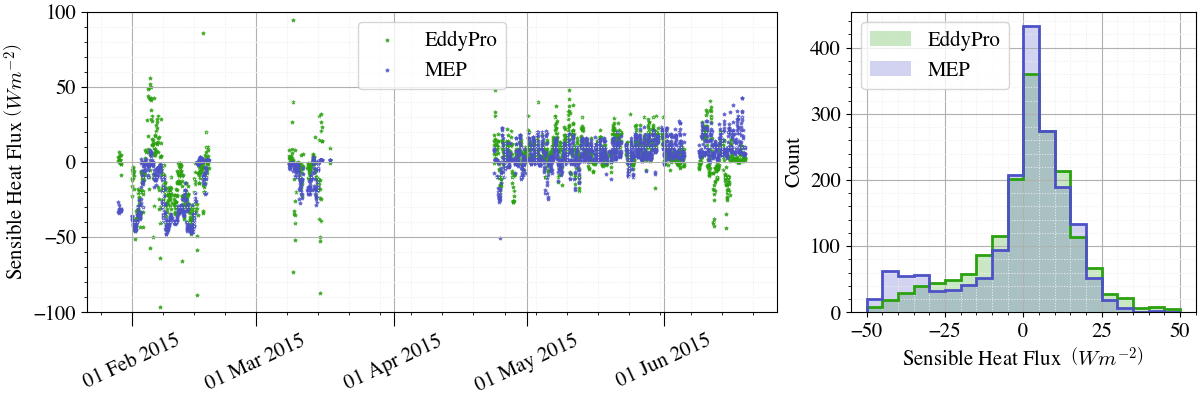
\includegraphics[width=1\linewidth]{figures/chapter3/MEPSensible.png}
    \caption[Sensible heat flux from the MEP method compared to EddyPro]{The sensible heat flux at N-ICE as calculated with EddyPro (green) and with the MEP method (blue).}
    \label{fig:mep:sensible}
\end{figure}

\begin{figure}[H]
    \centering
    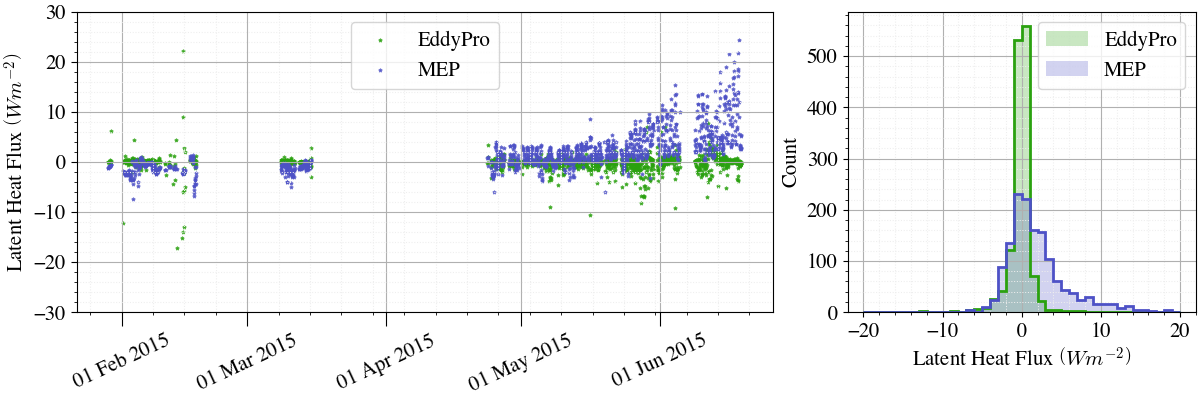
\includegraphics[width=1\linewidth]{figures/chapter3/MEPLatent.png}
    \caption[Latent heat flux from the MEP method compared to EddyPro]{The latent heat flux at N-ICE as calculated with EddyPro (green) and with the MEP method (blue).}
    \label{fig:mep:latent}
\end{figure}

Sensible heat flux from the MEP method is obtained using equation \ref{eq:mep:hs}. The results of this are shown in figure \ref{fig:mep:sensible}. The results using this method accurately represented the sensible heat fluxes at N-ICE for most of the experiment. In the winter, fluxes were slightly underestimated by the MEP equation, resulting in a bi-modal shape to the distribution shown on the right of the figure. In the spring, there was one occurrence lasting several days with largely negative sensible heat flux shown in the EddyPro results wile the sensible heat fluxes from the MEP equation stayed positive. 

Latent heat fluxes (figure \ref{fig:mep:latent}) were not represented as closely in the MEP to the EddyPro output. EddyPro showed very small latent heat fluxes throughout the entire experiment. These small heat fluxes were surprising and are not captured with the MEP method. February and March values of latent heat flux are comparable between the MEP and EddyPro calculations, but during spring and entering summer MEP values are at times $20 Wm^{-2}$ greater than those calculated by EddyPro, which are rarely greater than $10 Wm^{-2}$.

 \subsection{Bulk Flux Algorithm}
\begin{figure}[H]
    \centering
    \includegraphics[width=1\linewidth]{figures/chapter3/BulkSensible.png}
    \caption[Sensible heat flux from a bulk flux method compared to EddyPro]{The sensible heat flux at N-ICE as calculated with EddyPro (green) and with a bulk flux algorithm method (blue).}
    \label{fig:bulk:sensible}
\end{figure}
\begin{figure}[H]
    \centering
    \includegraphics[width=1\linewidth]{figures/chapter3/BulkLatent.png}
    \caption[Latent heat flux from a bulk flux method compared to EddyPro]{The latent heat flux at N-ICE as calculated with EddyPro (green) and with a bulk flux algorithm method (blue).}
    \label{fig:bulk:latent}
\end{figure}

Calculating the fluxes using the bulk flux algorithm resulted in more largely positive values than was represented in the EddyPro results and in the MEP results. These can be seen in figure \ref{fig:bulk:sensible}. In spring the sensible heat flux is consistently over estimated by the Bulk algorithm, indicating the temperature difference between the surface and the atmosphere is too large in the calculations, and too much head is being transferred in to the surface. The latent heat flux, shown in figure \ref{fig:bulk:latent}, was also calculated to be significantly larger than the EddyPro results when using the bulk flux algorithm. 

In June, there was a large decrease in the latent heat flux according to the bulk algorithm. This was mirrored by an increase in the sensible heat flux. However, this decrease (increase) in the latent heat flux (sensible heat flux) was not shown in the EddyPro method. EddyPro produced latent heat flux values consistently around zero during this time period, while the sensible heat flux dropped. This indicates that the air was cooler than the surface and sensible heat transfer occurred instead of a phase change. However, the bulk flux algorithm favored a phase change, likely melting, over a sensible heat flux change. At this time in the experiment, there likely was significant phase change occuring as many melt ponds were developing in the surrounding area \cite{walden:2017}. Overall, latent heat flux values estimated by the Bulk equation are more largely positive in the winter and more largely negative in the summer, indicating the Bulk flux algorithm shows more melting in the spring and more freezing in the winter than the EddyPro results. 

Positive latent heat flux values in the winter represent surface freezing. These values are, at times, almost $10 Wm^{-2}$ greater in the Bulk results than in the EddyPro results. EddyPro, once again, favors sensible heat flux changes to phase change. However, the sensible heat flux in the bulk algorithm and in EddyPro are comparable. This indicates that EddyPro is not just favoring the heat transfer to be in the form of sensible heat flux, but it also underestimates the latent heat flux in general, even in situations when it cannot be described by an offset in the sensible heat flux. 

%% SENSIBLE
% positive - surface warming (air warmer than sfc) if sfc correct air too warm
% negataive - surface cooling (air cooler than sfc) if sfc correct air too cold

%% LATENT
% positive - freezing
% negative - melting

\section{Summary and Conclusions}
Sensible and latent heat flux formulations require high temporal resolution to use eddy covariance methods. Two methods of calculating sensible and latent heat flux that do not require and eddy covariance measurements are explored here. The MEP method, a method utilizing the thermal conductivity, net radiative flux, and  the stability. The bulk flux method requires measurements of moisture and temperature at two levels, the wind speed, and stability. Both equations require the bulk transfer coefficients of heat and moisture, which are a function of the stability and have been empirically defined for experiments over a variety of surfaces. Very few of these functions are appropriate for the strong stabilities that often occur in the polar regions. Andreas et al., \cite{andreas:311} developed a relationship for these functions that applies to strong stabilities seen at SHEBA over multi-year sea ice. This relationship was found to be appropriate for the bulk transfer coefficients at N-ICE using both the bulk flux method and the MEP method. 

The MEP method performed well when compared to the EddyPro values for both sensible and latent heat fluxes. In the winter, the latent heat flux values calculated by the MEP equation are much higher than those in EddyPro, indicating significant more phase change. The bulk method also represented the EddyPro values fairly well, though the MEP formulations does seem to represent the spread of flux values better than the bulk algorithm. The latent heat flux values were also much larger than those observed during N-ICE in the bulk method. 

Overall, further testing is needed for validation of the latent heat flux formulations. The latent heat flux values measured at N-ICE were much smaller than expected, and smaller than those seen at other experiments, so more measurements are needed to determine if this is something that can be expected. Both sensible heat flux formulations, however, produced reasonable values over the first-year sea ice seen at N-ICE. 
  \chapter{Cloud macrophysical and radiative properties observed during the Norwegian Young Sea Ice field campaign}
\vspace{1 cm}
\begin{spacing}{1} \begin{quote} 
\noindent \emph{The combined effect of all climate feedback processes is to amplify the climate response to forcing (virtually certain). While major advances in the understanding of cloud processes have increased the level of confidence and decreased the uncertainty range for the cloud feedback by about 50$\%$ compared to AR5, clouds remain the largest contribution to overall uncertainty in climate feedbacks (high confidence).} \end{quote}
\hspace{6 cm} - IPCC Sixth Assessment Report, August 2021  
\end{spacing}
\doublespacing
\section{Introduction}
The global climate is heavily influenced by processes that occur in the Arctic. However, the Arctic environment is currently experiencing rapid change \citep{overland:2011, stroeve:2007}. Due to a lack of observations, it has been difficult to fully understand atmospheric processes in the polar regions \citep{persson:2002}. The atmospheric circulation in the Arctic is modified by changes in the overall climate, which, in turn, impact cloudiness and radiation at the surface \citep{zhang:2008}. The Advanced Very High-Resolution Radiometer (AVHRR) has observed that wintertime cloud cover over the Arctic Ocean is decreasing by 5$\%$ per decade. Meanwhile, in spring, increases as large as 15$\%$ per decade have been observed, which can likely be attributed to changes in atmospheric circulation \citep{schweiger:2004}. A decreasing trend in Arctic sea ice of -2.9$\%$ to -9.1$\%$ per decade was seen from 1979 through 2006 \citep{stroeve:2007}. Measurements of the energy balance and cloud properties (fraction, height, microphysical, and temperature) can give important insight into climate processes and radiative transfer but are rarely measured together \citep{persson:2002, schweiger:2004, miller:2017}. 

Clouds change the surface temperature by modifying both the shortwave and longwave radiation reaching the surface. Cloud microphysics, such as phase and particle size, as well as macrophysics, including fractional coverage, cloud height, and thickness, can influence the amount of radiation reaching the surface and, in turn, influence the impact of the cloud-radiation feedback \citep{uttal:2002}. This relationship is nonlinear and depends on both cloud and sea ice characteristics \citep{intrieri:2002}.

Clouds, as stated above, can modify both the radiation budget and impact the ice-albedo feedback. The influence of clouds is magnified by the high surface albedo and the lack of atmospheric moisture \citep{shupe:2003}. Clouds have the greatest potential to modify heat exchange in the Arctic \citep{intrieri:2002}. While we do have some estimates on how much the clouds can impact these feedbacks, more information is needed to quantify the exact influence. \citet{sledd:2019} states that the clouds are the most important driver in changes in top-of-atmosphere albedo over the entire globe, including at the poles, regardless of the high surface albedo. Cloud characteristics were shown to directly impact the ice thickness in studies by \citet{curry:1992, beesley:2007}.  

The impact of clouds is often quantified using cloud radiative forcing (CRF). The CRF describes how clouds modify the radiation at the surface by taking the difference between the observed all-sky radiation and the estimated clear-sky radiation \citep{ramanathan:1989}. When positive radiative forcing is observed, there is a surplus of net radiation at the surface under cloudy skies, and they drive warming. When the CRF is negative, cooling occurs at the surface under clouds. During clear skies, CRF should equal zero, as the actual radiation should be the same as the estimation of clear-sky radiation. Clear-sky radiation is often calculated from a radiative transfer model or estimated using observed clear-sky times.

Net cloud radiative forcing is a balance of surface warming and cooling due to modifications in radiation as a result of cloud cover. \citet{curry:1992, intrieri:2002} found that in the Arctic, clouds warm the surface over the entire year (have a positive cloud radiative forcing) except for in mid-July, when the sun is high above the horizon and the surface albedo is relatively low. This nearly year-round warming is due to the small amount of shortwave radiation. When there is solar radiation present, the low sun elevation angle and high surface albedo reflect much of the shortwave radiation away. In addition, the low-level clouds are often emitting longwave radiation at warmer temperatures than the ice surface due to surface temperature inversions \citep{shupe:2003} and are always emitting more effectively than the clear sky.

The Norwegian Young Sea Ice Experiment (N-ICE2015, or N-ICE) \citep{granskog:2018} is the first experiment to make comprehensive measurements of clouds and the surface energy balance from winter to summer since the Surface Heat Budget of the Arctic Ocean Experiment (SHEBA) in 1997 and 1998 \citep{walden:2017, uttal:2002}. While N-ICE was conducted north of Svalbard in the Arctic Ocean, SHEBA took place north of Alaska in the Beaufort and Chukchi Seas, measuring the components surface energy budget \citep{persson:2002, andreas:2010, grachev:2007}, cloud properties \citep{turner:2005, turner:2002, intrieri:2002, shupe:2004}, and the resulting surface properties \citep{intrieri:2002, shupe:2004}. 

SHEBA was conducted almost two decades before N-ICE. Measurements were taken further into the ice pack \citep{cohen:2017} and in thicker ice conditions. In addition, the meteorological conditions were different; detailed comparisons of N-ICE and SHEBA during the winter can be found in \citep{graham:2017}. There were a few warm events during N-ICE caused by synoptic storms when temperatures reach 0 $^{\circ}C$; these events were much warmer than any of the warm periods experienced during SHEBA.  During the warm periods at N-ICE, the cloud properties were quite variable, suggesting that some of the changes in the surface energy balance could be the result of changes in cloud macrophysical and/or microphysical properties. Throughout SHEBA, mixed-phase clouds were observed 41$\%$ of the time. \citet{graham:2017} states that in the winter, extreme radiative cooling events were more frequent during the N-ICE period than during SHEBA. More information about N-ICE can be found in Chapter 2.

Due to their importance to the surface energy budget over the Arctic Ocean, it is important to investigate the properties and radiative forcing of clouds during N-ICE and to compare the results to those observed during SHEBA. These results will provide useful constraints for models that traditionally have had difficulty simulating radiation at the surface of Arctic sea ice. Proper modeling of Arctic clouds in all seasons is essential for simulating accurate values of the surface energy budget, which is critical for modeling the seasonal cycle of sea ice. A critical parameter that was identified during SHEBA \citep{inoue:2008, tjernstrom:2005} and other Arctic field experiments \citep{hines:2017, listowski:2017, hines:2019} is the fraction of mixed-phase clouds. \citet{graham:2017} showed that six atmospheric reanalyses have difficulty simulating Arctic clouds.

This paper uses various observations obtained during the N-ICE2015 field campaign to document the cloud macrophysical properties, the shortwave (SW) and longwave (LW) radiation, and the net cloud radiative forcing (CRF) at the surface of young Arctic sea ice. Section 2 describes the various measurements that were made during N-ICE to estimate CRF. Section 3 describes the methods to calculate CRF, which involved combining N-ICE measurements with radiative transfer modeling. Section 4 describes the seasonal transition of CRF from winter to summer. Section 5 compares the calculated CRF to modeled CRF in two model simulations. Section 6 presents the conclusions of this study.

\section{Measurements}
N-ICE was conducted during the six-month transition from winter to summer (January - June 2015) in the Arctic Ocean north of Svalbard. All of the instruments were either deployed onboard the Norwegian research vessel Lance or on the sea ice near the Lance. The instruments used in this study were a Vaisala CL-25 ceilometer, a Micropulse Lidar (MPL), twice-daily Vaisala RS92-SGP radiosondes, and Kipp and Zonen shortwave and longwave broadband radiometers. More information about N-ICE can be found in Chapter 2. 

The synoptic context of the N-ICE field campaign is described by \citet{cohen:2017}. The storms designated in Table 2 of \citet{cohen:2017} are of particular interest to this study. Six major and three minor storms occurred in winter (between 21 January and 14 March), while two major and seven minor storms occur in spring and summer (from 23 April through 11 June). The winter was characterized by a succession of particularly strong storms (as compared to climatology), while the spring conditions were typical of that region of the Arctic \citep{graham:2017}. The winter storms were accompanied by large increases in the integrated water vapor and changes in wind direction \citep{kayser:2017} that influenced cloud properties.

A list of the meteorological instrumentation deployed during N-ICE is given in Table 1 of \citet{cohen:2017}. A thorough description of the Vaisala RS92-SGP radiosondes launched during N-ICE is given by \citet{kayser:2017}. A brief description of the meteorological measurements is given here as they pertain to this study.

Radiosondes were launched from the ice surface (Floe 1) and from the ship deck (Floes 2, 3, 4) to measure vertical profiles of temperature, relative humidity, wind speed and direction, pressure, and geopotential height up to a maximum altitude of 30 $km$. More information and analysis of the radiosondes can be found in \citep{kayser:2017}. Here the radiosonde profiles were combined with the surface and tower meteorological measurements to create input files for a radiative transfer model (section 3.2).

A MPL was used to measure backscattered radiation and depolarization from aerosols and clouds along the vertical path of the lidar beam throughout the N-ICE field campaign \citep{spinhirne}. The MPL was mounted on the upper deck of the R/V Lance and was approximately 10-12 meters above the sea ice surface \citep{campbell:2002}. The MPL is a Sigma Space Version 4 polarization-sensitive lidar (532 $nm$) that was provided by the U.S. Department of Energy’s (DOE) Atmospheric Radiation Measurement (ARM) Program. Raw MPL data was collected at 5-second temporal resolution and 15-meter spatial resolution up to an altitude of 18 km above the surface. The uncertainty in the base height of clouds (derived from MPL measurements) is $\pm$ 2 $\%$ due to timing uncertainties within the instrument. The lidar beam is attenuated more by water droplets than ice particles, so our determination of the cloud fractions of water and ice clouds is biased toward a higher percentage of water than ice. In addition, the MPL signal is highly attenuated by optically thick clouds, so when a low thick water cloud is detected, it is possible that additional cloud layers may exist above this layer that is not detected by the MPL. In these cases (which occur often in spring and summer), we assume that the low thick cloud layer is solely responsible for the cloud radiative forcing at the surface. Post-processing of the MPL measurements is described below in section 3.1 and is based on the analysis methods of \citet{campbell:2002}, \citet{flynn:2007}, and \citet{stillwell:2018}.

Broadband radiometers were deployed at 1 to 1.2 $m$ above the surface near the meteorological tower to measure upward and downward components of longwave (Kipp and Zonen CGR4) and shortwave (Kipp and Zonen CMP22) radiation. Kipp and Zonen CVF4 ventilation units were used to heat and ventilate the radiometers to avoid frosting of the instrument domes during periods of high relative humidity. The surface skin temperature was calculated from the upwelling and downwelling longwave radiation, assuming a broadband surface emissivity of 0.99 \citep{grenfell:1999}; the surface skin temperature was used as input for radiative transfer modeling. More information about the radiometers, including analysis of the surface energy budget, can be found in \citet{walden:2017}.

In spite of deploying a relatively comprehensive instrument suite over sea ice during N-ICE2015, there are some caveats regarding these measurements. Most importantly, when the optical depth of the overlying clouds is large, the MPL is unable to penetrate completely through the clouds. This is especially true when liquid water clouds are present, which occur often in spring and summer and occasionally in winter. Thus, the cloud macrophysical properties that are reported here represent only the lowest layer of cloud cover in many cases. It would have been preferable to also deploy a cloud radar, which is less sensitive to liquid water, that would have profiled clouds above any liquid layers. Other additional instruments would have been useful for measuring the liquid water path (microwave radiometer) and cloud microphysical properties (infrared spectrometer, cloud radar). So given the instruments that were deployed, we report on both the cloud macrophysical properties (within the capability of the MPL) and cloud radiation, with a focus on surface cloud radiative forcing, which is most sensitive to the lowest cloud layer. 

\section{Methods}
In this study, the macrophysical and radiative properties of clouds are described throughout the N-ICE2015 field campaign. Below we explain how cloud base height, temperature, fraction, and cloud radiative forcing are derived from the instruments deployed during the field campaign.

\subsection{Cloud Macrophysical Properties}
Measurements from the MPL and routine radiosonde launches during N-ICE provide estimates of three macrophysical cloud properties: cloud fraction, temperature, and phase. Raw data from the MPL were corrected for pulse pileup (saturation) and background light (from sky and/or detector dark noise), creating “background-subtracted raw counts”. Several additional corrections are then applied: afterpulse calibration, daily normalization to the median laser pulse energy, and an overlap correction to remove the effect of range-dependent collection efficiency of the fiber-coupled receiver  \citep{campbell:2002, micropulse:2006}. Both signal-to-noise (SNR) and speckle filtering was then performed on the data.

Two lidar parameters are then calculated for our analysis: backscatter ratio and polarization. The backscatter ratio is the ratio of total backscattering to molecular backscattering \citep{klett:1981}. The molecular backscattering is estimated using twice-daily radiosonde data. The radiosonde profiles of pressure, temperature, and water vapor were interpolated in time and space to approximate molecular particle number density. Molecular backscattering was then calculated using the Rayleigh scattering approximation \citep{bohren:2006, bohren:2008, placzek:1934}. 

In this study, the backscatter ratio for each lidar volume pixel is used to distinguish clear air from liquid or ice hydrometeors. A volume pixel, or voxel, is a lidar measurement at a particular time and altitude range. Backscatter ratios greater than 7.5 were considered cloudy voxels, while ratios less than 7.5 were identified as clear voxels (that may or may not contain aerosols). The cloud-base height is the lowest altitude a cloud is detected, and the cloud top is the highest. As mentioned above, if the optical depth of the lowest cloud is large, the MPL will only accurately detect the base of the lowest cloud. Once the cloud base is determined, the cloud temperature can be estimated by interpolating the twice-daily radiosonde profiles to the particular time and altitude of the cloud base. The cloud fraction (occurrence) for a given time period is then determined by calculating the fraction of time when a cloud is present vertically overhead.

The polarization of the MPL is calculated using equations 1.4 (depolarization ratio) and 1.5 (depolarization) of \citet{flynn:2007}. These parameters, plus the error in the depolarization ratio, are used to classify the cloudy voxels into three categories: liquid, ice, and unclassified cloud. Cloudy voxels with depolarization ratios greater than 0.1 are classified as ice, while voxels with depolarization ratios lower than 0.1 are liquid. Cloud voxels cannot be classified as mixed-phase and are conservatively categorized as liquid versus ice as done in previous lidar studies (e.g., \citet{intrieri:2002}). The classification is further refined using the error in depolarization ratio, requiring this error for liquid and ice to be less than 10 $\%$. If the depolarization-ratio error is greater than 10 $\%$ for the initial classification of liquid or ice, the cloud voxel is classified as an “unclassified cloud”. 

Once each voxel is classified, a column cloud mask is created for comparing the range-resolved lidar measurements with the column measurements made by the broadband radiometers. If the atmospheric column above the lidar lacks clouds at any altitude, the column is considered clear, otherwise, the column is cloudy. Columns containing liquid voxels at any altitude are considered liquid. This implies that a single liquid voxel can override numerous ice voxels. This is done because liquid clouds in the Arctic typically have large optical depths (e.g., \citet{curry:1996}) relative to ice clouds.

\subsection{Cloud Radiative Properties}
The all-sky net radiation at the surface $Q_{all}$ is calculated using 1-hour average radiation measurements from the four Kipp and Zonen radiometers, where the $Q_{all}$ is defined in Eq. \ref{eq:qnet}. $Q_{all}$ is equal to $Q_{net}$ for observations.

\begin{equation}\label{eq:qnet}
Q_{all} = (Q_{lw \downarrow} - Q_{lw \uparrow}) + (Q_{sw \downarrow} - Q_{sw \uparrow})
\end{equation}

$Q_{lw \downarrow}$, $Q_{lw \uparrow}$, $Q_{sw \downarrow}$ and $Q_{sw \uparrow}$ are the components of downward longwave, upward longwave, downward shortwave and upward shortwave radiation. In this paper, positive net radiation is defined as into the surface \citep{miller:2015}.

Cloud radiative forcing is defined in Eq. \ref{eq:crf:1}, \ref{eq:crf:2}, and \ref{eq:crf:3} \citep{ramanathan:1989, miller:2015}.

\begin{equation}\label{eq:crf:1}
CRF = Q_{all} - Q_{clear}
\end{equation}
\begin{dmath}\label{eq:crf:2}
CRF = [(Q_{lw \downarrow} - Q_{lw \uparrow}) + (Q_{sw \downarrow} - Q_{sw \uparrow})]_{all} \\
\\ - [(Q_{lw \downarrow} - Q_{lw \uparrow}) + (Q_{sw \downarrow} - Q_{sw \downarrow})]_{clear}
\end{dmath}
\begin{dmath}\label{eq:crf:3}
CRF = [(Q_{lw \downarrow} - Q_{lw \uparrow})_{all} - (Q_{lw \downarrow} - Q_{lw \uparrow})_{clear}] \\
\\ + [(Q_{sw \downarrow} - Q_{sw \uparrow})_{all} -  (Q_{sw \downarrow} - Q_{sw \uparrow})_{clear}]
\end{dmath}

The clear-sky values for both downward longwave and shortwave radiation in Eq. \ref{eq:crf:3} are calculated using the Rapid Radiative Transfer Model (RRTM) \citep{mlawer:1997} because there were too few clear-sky cases during N-ICE2015 to properly estimate the clear-sky flux using the radiation measurements. For SW calculations, it is important to specify the atmospheric concentrations of $N_{2}$ and $O_{2}$ for molecular scattering and $H_{2}O$, $O_{3}$ and $O_{2}$ for molecular absorption. The surface albedo must also be specified as a function of the surface type and solar zenith angle. For LW calculations, the vertical temperature structure must be specified, as well as the concentrations of the primary infrared greenhouse gases ($H_{2}O$, $CO_{2}$, $O_{3}$, $CH_{4}$, $N_{2}O$, $CO$).

 It is important to specify a vertical grid in RRTM that resolves the near-surface temperature structure because near-surface temperature inversions occurred during N-ICE \citep{kayser:2017}. Here we use three layers (surface, 2 $m$, 4 $m$) below 10 $m$, then increasing spacing above 10 $m$: 10 $m$ spacing from 10 to 100 $m$, 100 $m$ from 100 $m$ to 1 $km$, 1 $km$ from 1 to 30 $km$, and 5 $km$ from 30 to 60 $km$. RRTM was run hourly for the entire field campaign.

Here the concentrations of $N_{2}$ and $CO_{2}$ are assumed to be uniformly mixed vertically, while the seasonal variability of the $CO_{2}$ concentration is accounted for by using monthly averaged measurements from Summit Station, Greenland made by the Global Monitoring Division (GMD) from National Oceanic and Atmospheric Administration (NOAA). The profiles of $O_{2}$, $CH_{4}$, $N_{2}O$, and $CO$ are from the sub-Arctic winter standard atmosphere \citep{mcclatchey:1972}. The profiles of $O_{3}$ were measured at Ny-\r{A}lesund, Svalbard, and were interpolated to hourly profiles. The profiles of temperature and humidity were constructed using: 1) the sensors at 2 $m$ and 4 $m$ on the meteorological tower, 2) the radiosondes from 10 $m$ to the altitude of the balloon burst, and 3) values from the sub-Arctic winter standard atmosphere from the maximum altitude of the radiosonde to 60 $km$. On a few occasions, the termination height of the radiosonde was low (below 10 $km$). In these cases, the monthly average sonde profiles were used from the maximum altitude of the sonde through 24 to 30 $km$ depending on the month. The surface skin temperature was derived from the longwave radiation \citep{walden:2017} and assumed a surface snow emissivity of 0.98 \citep{persson:2002, grenfell:1999}.

The meteorological tower data were compared to the lowest 10 $m$ measured by the radiosondes as a quality check because of the strong dependence of longwave CRF on the near-surface temperature structure. The difference between the 2$-m$ temperature measured on the meteorological tower and the temperature interpolated between radiosondes exceeded 1$^{\circ}C$ in only 1.2$\%$ of the hourly profiles. The other levels (2, 4, and 10 $m$) exceeded a 1$^{\circ}C$ difference of less than 0.5$\%$ of the time. To ensure the lower profiles were as accurate as possible, the tower temperatures and surface temperatures calculated from LW fluxes were used when available but did not change the lower levels of the profiles significantly. Linear interpolation between the tower and sonde measurements was sufficient to represent the lower atmosphere because the altitude range of these temperature adjustments was small ($<$10 $m$).

\begin{figure}[b!]
    \centering
    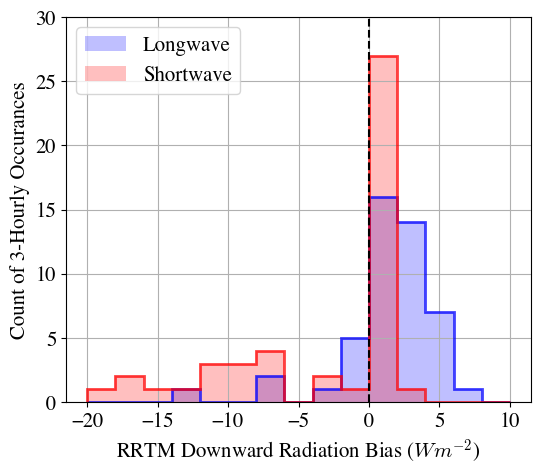
\includegraphics[width=0.65\linewidth]{figures/chapter4/RRTMcorrelation_bias.png}
    \caption[RRTM modeled downward flux bias histogram.]{RRTM modeled downward longwave flux bias (RRTM - observations) in blue and downward shortwave flux bias in red. Three-hourly values during clear-sky times only are shown.}
    \label{fig:rrtm}
\end{figure}

The shortwave spectral surface albedo was estimated using the snow albedo model described by \citet{wiscombe:1980}; see their Eq. 4. This model depends on properties of the snow (single-scattering albedo ($\omega$) and asymmetry factor ($g$)), as well as the solar zenith angle ($\theta$). The single-scattering albedo was determined for each day using noontime albedo measurements from \citet{walden:2017}. A fixed value of $g$ = 0.9 was used. These values were then used along with the hourly solar zenith angle to calculate the albedo throughout the day. The cloud cover also greatly affects the surface albedo, and this was parameterized using a diffuse fraction. \citet{key:2001} states that the albedo of ice is 4 to 6$\%$ higher under cloudy skies than clear skies with a range of 0 to 15$\%$. Cloud fraction for the two-hour period surrounding the time of the albedo calculation was used to determine the percent reduction required to account for the diffuse fraction. Percent reductions in albedo were scaled linearly from 6 to 0$\%$, with full cloud cover having a 6$\%$ reduction imposed, and clear sky remaining unchanged.

Uncertainties are introduced into RRTM shortwave and longwave calculations from uncertainties in the albedo estimates, atmospheric profile construction and interpolation, and the various measurements. Despite this, the RRTM calculations agree well with the few clear-sky SW and LW measurements from N-ICE2015. Figure \ref{fig:rrtm} shows a histogram of the differences in SW and LW radiation (modeled minus measured) for clear days. The mean SW bias is -2.5 $W m^{-2}$ with a standard deviation of 9.6 $W m^{-2}$, while the mean LW bias is 1.3 $W m^{-2}$ with a standard deviation of 3.6 $W m^{-2}$. Thirteen three-hour periods that appeared clear in the data were removed as they were at the start of an observation period (the beginning of a floe). These periods had significant differences but, because these were some of the first measurements during their respective floes, they were removed due to the potential for instrument error.

\section{Results and Discussion}
The conditions observed at N-ICE were unique not only because it observed the transition season for the first time since SHEBA. Winter storm periods were measured that brought extremely large and rapid transitions of cloud properties that coincide with changes in turbulent fluxes documented by \citet{walden:2017} and \citet{graham:2017}. 

\begin{figure}[t!]
    \centering
    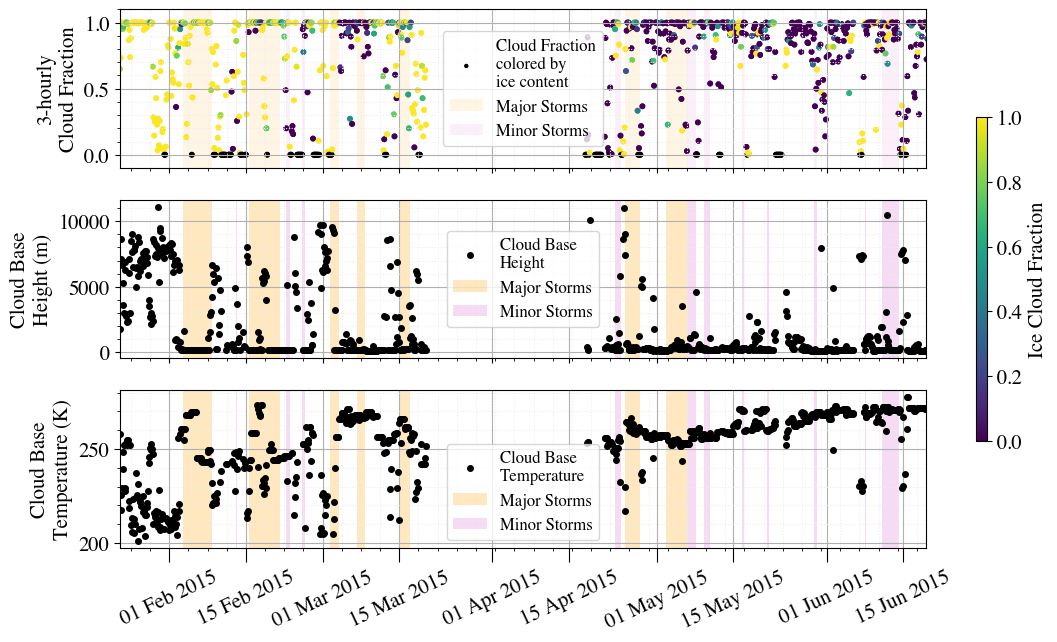
\includegraphics[width=1\linewidth]{figures/chapter4/CloudSummary.png}
    \caption[Cloud fraction and phase, height, and temperature time series.]{Vertical cloud fraction and ice content within the cloud are shown in the top figure. Ice content is defined as the percentage of the cloud that can be determined to be ice particles (yellow represents more ice and purple less). The middle panel shows the 3-hourly mean cloud base height and the bottom panel shows the 3-hourly cloud base temperature. Storm periods are shaded in orange (major) and pink (minor) shading.}
    \label{fig:cloudmacro}
\end{figure}

The upper panel of Figure \ref{fig:cloudmacro} shows the vertical cloud fraction, or the percentage of the day that cloud was observed over the MPL, indicated by colorful dots. The color indicates the ice cloud fraction or the percentage of the observed clouds that could be definitively categorized as ice. During the first half of the experiment in winter, it was common for days to have cloud fractions below 50$\%$, with 16 out of the 61 days prior to the long break in observations having less than 50$\%$ cloud cover. After the break, however, there are only 12 days out of the 89 days that are below 50$\%$ cloud cover. The mean cloud fraction during the first half of the experiment is 70$\%$ (standard deviation of 30$\%$), and after is 75$\%$ (standard deviation of 28$\%$). Climatologically, a decrease in clear days has been seen for this region, contributing to a long-term warming trend \citep{kayser:2017}. The entire experiment, including a large number of cloudy days, is put into climatological context by \citet{graham:2017} and \citet{kayser:2017}. For the purpose of this study, there was significantly less cloud cover in winter than in the spring and summer, and the clouds observed during winter had larger ice content than those observed during spring.

During Floes 1 and 2 (winter), every day has at least some ice cloud present. Most of the days have primarily ice clouds with the exception of a week in early March, which corresponds to a period when the cloud base was low (Figure \ref{fig:cloudmacro}, middle panel) and cloud temperature was near freezing (265 - 270 $K$, Figure \ref{fig:cloudmacro}, bottom panel). Some days have a small percentage of unknown cloud fraction, but this category only exceeds 20$\%$ of the daily cloud existence once during the first half of the experiment. 

\begin{figure}[b!]
    \centering
    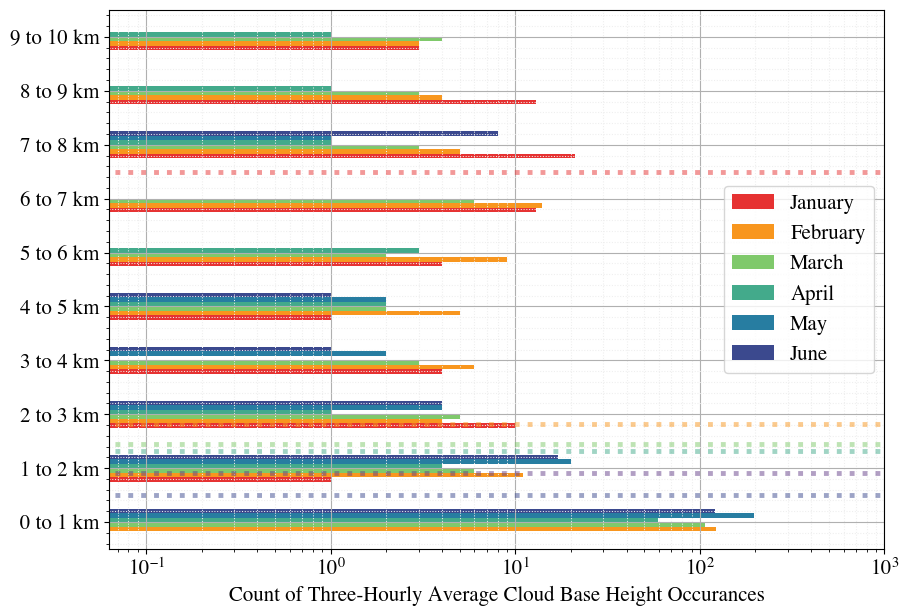
\includegraphics[width=1\linewidth]{figures/chapter4/CloudHeights.png}
    \caption[Cloud base height by month histogram.]{Binned cloud base height by month. Frequency distributions are shown as bars colored by month. The monthly mean cloud height is shown by the horizontal line in the corresponding color.}
    \label{fig:cloudbase}
\end{figure}

The fraction of water clouds greatly increases during Floes 3 and 4 (spring and summer). These results are not surprising, as increasing temperature and increasing water fraction are expected. There are still ice clouds present nearly every day through the end of the experiment, many of which are high, thin clouds. The water clouds, however, were primarily thick and close to the surface. Some of the ice can be attributed to mixed-phase clouds with both water and ice through the mid-troposphere. Low-level ice clouds were not common during this period.

Cloud base heights (Figure \ref{fig:cloudmacro}, middle panel) in the first month of the experiment are, on average, higher than the rest of the experiment. Once Floe 3 starts cloud base heights are almost always below 2 $km$. Figure \ref{fig:cloudbase} shows the frequency of cloud base heights for each month throughout the experiment with lines indicating the mean cloud base height. The mean height for January, which includes only a 10-day, relatively quiescent period, is 6.45 $km$, while the rest of the months' mean cloud heights are below 2 $km$. Mean cloud heights decrease throughout the experiment, with the lowest mean cloud base height present in May at just below 1 $km$. During the second half of the experiment, the majority of the clouds have a low cloud base height and a high percentage of water present. These clouds had large enough optical depths that they caused complete attenuation of the micropulse lidar beam, resulting in an inability to view clouds above them. As mentioned above, this inhibits the ability to report on higher-level clouds but does not impact the ability to understand the surface energy budget, as these low-level clouds are the most radiatively important.

Cloud base temperature closely mimics the cloud base height for the majority of the experiment. During the second two floes, the cloud base temperature gradually approaches freezing while the cloud base height stays fairly consistently near the surface. This slow increase in cloud base temperature reflects the increase in atmospheric temperature as more solar radiation reaches the Arctic. 

\subsection{Cloud Radiative Properties}
This section describes the variations in shortwave and longwave fluxes measured throughout N-ICE2015. These fluxes are used to calculate the shortwave, longwave, and net CRF throughout the campaign as defined by Eq. \ref{eq:crf} above. These measurements are then categorized according to the cloud macrophysical properties described above.

\begin{figure}[h]
    \centering
    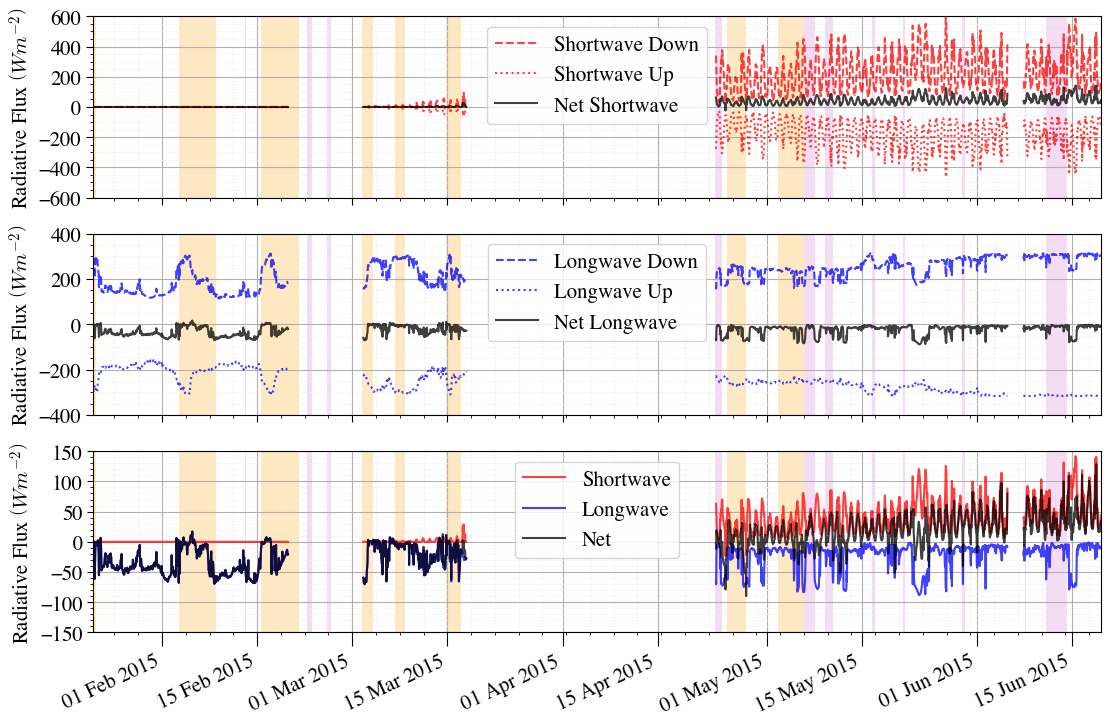
\includegraphics[width=1\linewidth]{figures/chapter4/RadComp.png}
    \caption[Shortwave, longwave, and net radiative components of flux.]{Shortwave (top), longwave (middle), and net (bottom) components of radiative flux. Black lines represent net flux, dotted indicating upward flux, and dashed downward. Major and minor storm periods are shown by the orange and pink shading, respectively.}
    \label{fig:flux:all}
\end{figure}

Figure \ref{fig:flux:all} shows the time series of the shortwave (upper panel), longwave (middle panel), and net (lower panel) radiative fluxes. During Floe 1 (January and February), net flux (also, net longwave flux) dips to around -50 $Wm^{-2}$ during non-storm periods (unshaded) and approaches 0 $Wm^{-2}$ during storm periods (shaded). During major winter storms, downward longwave flux increases from between 100 and 150 $W m^{-2}$ to around 300 $Wm^{-2}$, sometimes within only a few hours. Upward longwave flux mirrors these changes decreasing from -200 to -300 $Wm^{-2}$. During non-storm periods, the upward flux is around -200 $Wm^{-2}$ while the downward flux is just over +100 $Wm^{-2}$, resulting in negative net flux. When the net flux approaches zero, as it does during storm periods, it indicates that clouds are relatively low and warm and have a large enough optical thickness to balance the longwave flux coming from the surface.

In March (Floe 2), the downward and upward longwave fluxes more closely balance each other. This is due to a generally higher downward longwave flux from warmer cloud base temperatures and higher optical thicknesses from a greater fraction of liquid water clouds (Figure \ref{fig:cloudbase}, top panel). During non-storm periods, the net longwave flux reaches a minimum just below -50 $Wm^{-2}$ but is more frequently around -25 $Wm^{-2}$. Storm periods continue to bring the net flux near 0 $Wm^{-2}$, as lower and warmer clouds predominate. Small amounts of shortwave flux exist during the end of this floe (net $< 50~Wm^{-2}$) as the sunlight returns to these latitudes, but has little influence on net flux due to a large amount of reflected shortwave flux from the surrounding snow.

During Floe 3 (spring), the net longwave flux reaches as low as -70 $Wm^{-2}$ but is more often around 0 $Wm^{-2}$. This is the result of increased and consistently high downward longwave flux. This is when the atmosphere is in an opaquely cloudy state \citep{stramler:2011, graham:2017}. As the experiment transitioned from winter into spring, cloud base height decreased and cloud occurrence increased. The decrease in cloud height and warming of the atmosphere results in an increased downward longwave flux from the clouds. In addition, during this period, the floe drifted into warmer ocean water \citep{kayser:2017} and the net shortwave flux increased, which increased the atmospheric temperature above the ice and the magnitude of the upward longwave flux. Upward longwave radiation is fairly consistent throughout this floe, starting around -225 to -250 $Wm^{-2}$ in late April and steadily increasing in magnitude to around -300 $Wm^{-2}$ in June. During this period, the upward longwave flux does not mirror the downward longwave flux as closely as it does during winter, especially as the surface temperature approaches freezing ($Q_{LW\uparrow} \approx 316~W~m^{-2}$).

The net shortwave flux during Floe 3 generally fluctuates between 0 and 100 $Wm^{-2}$, with only 6 days exceeding 100 $Wm^{-2}$. The total net flux follows the daily pattern of the net shortwave flux and is primarily greater than 0 $Wm^{-2}$. During the start of this floe, net flux drops below 0 $Wm^{-2}$ during the two major storm periods. These drops are caused by both a decrease in net shortwave flux (due to increased cloud optical thickness) and a decrease in net longwave flux (higher cloud base and lower cloud base temperature, Figure \ref{fig:cloudmacro}). After this, there are a few more occurrences in which the flux decreases below 0 $Wm^{-2}$, which coincide with decreases in the net longwave radiation, indicating higher cloud bases and/or lower cloud fractions (Figure \ref{fig:cloudmacro}).  

June (Floe 4) experienced the greatest magnitude of net flux. Only two days (23 May and 15 June) had a daily average flux larger than 350 $Wm^{-2}$. These days had primarily clear sky conditions. During the only spring storm period, net flux decreases significantly (from around 75 $Wm^{-2}$ to less than 50 $Wm^{-2}$) due to a decrease in downward shortwave flux. This occurs at the same time as an increase in cloud base height from near the surface to around 10 $km$ (Figure \ref{fig:cloudmacro}, middle panel). This is the largest decrease in net flux in June. During this time, optically thick clouds block shortwave radiation from reaching the surface. However, because these cloud bases were warm and close to the surface, net longwave flux rose to around 0 $Wm^{-2}$ during this time, keeping net flux above 0 $Wm^{-2}$. After the storm, net flux again drops to around the same magnitude as during the storm period, but this time accompanied by a decrease in downward longwave flux. This corresponds to an increase in cloud base height, a decrease in cloud base temperature, and a decrease in the cloud fraction (Figure \ref{fig:cloudmacro}) indicating that, after the storm passed, clouds became high and more scattered, including a day with the lowest cloud fraction in June. 

\begin{figure}[t!]
    \centering
    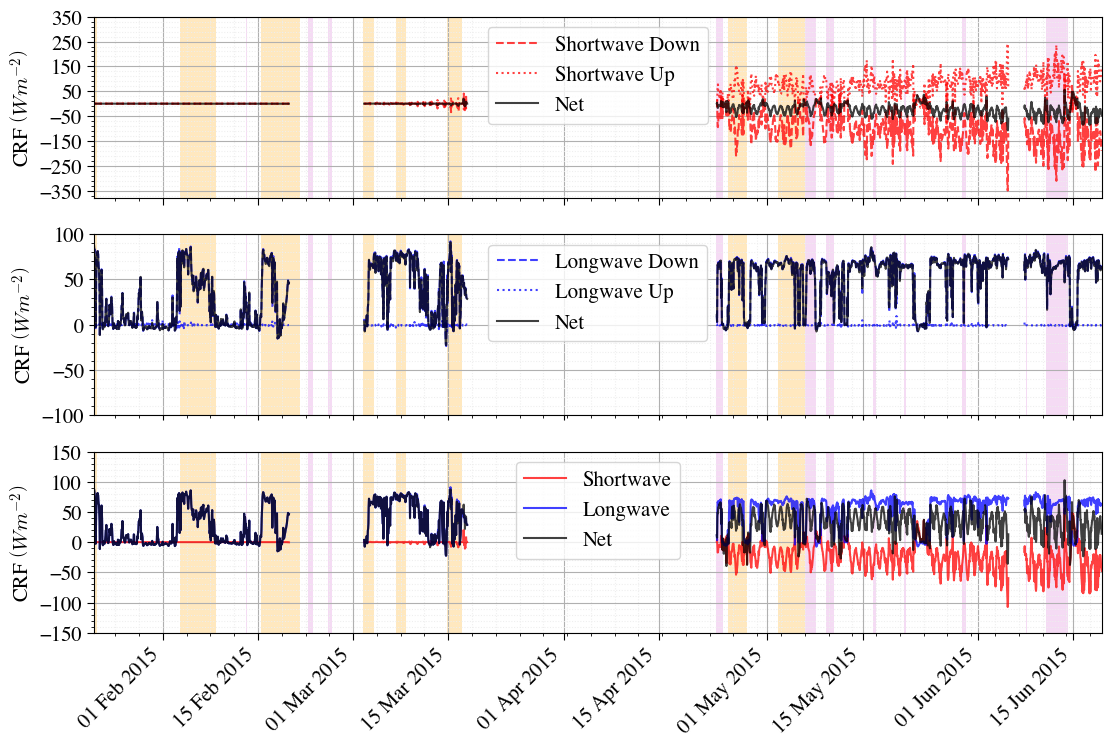
\includegraphics[width=1\linewidth]{figures/chapter4/RadForcing.png}
    \caption[Shortwave, longwave, and net components of cloud radiative forcing.]{Shortwave (top), longwave (middle), and net (bottom) components of cloud radiative forcing. Black lines represent net flux, dotted indicating upward CRF, and dashed downward. Major and minor storm periods are shown by the orange and pink shading, respectively.}
    \label{fig:crf_timeseries}
\end{figure}

Cloud radiative forcing at the surface is shown in Figure \ref{fig:crf_timeseries}. (Here CRF is defined to be positive if there is net energy gained \emph{into} the surface under clouds, compared to clear sky.) Longwave CRF dominates throughout the field campaign. During Floes 3 and 4, the shortwave CRF has an increasing influence on the net CRF, but only decreases it by a small amount. Upward and downward shortwave CRF counteract each other due to the high albedo of the snow cover on the sea ice, resulting in net shortwave CRF between -50 and 0 $Wm^{-2}$. (\citet{walden:2017} report values of the surface albedo during N-ICE2015.) It is important to note that the clear-sky modeled radiation was estimated to be slightly less than the measured radiation, resulting in clear-sky periods being slightly negative in some cases. This can be seen in the first floe when the upward longwave CRF is slightly below zero, creating a negative CRF. This does not mean that clouds were cooling the surface at this time. 

Due to the positive CRF throughout almost the entire field campaign, clouds are generally warming the surface. During SHEBA and other studies \citep{schweiger:2004, cogley:1984, walsh:1998, curry:1996} clouds were found to warm the surface throughout the entire year except in mid-summer when the solar zenith angle was high and albedo low. The length of this cooling period was highly dependent on albedo estimations \citep{intrieri:2002}. As N-ICE did not continue through the entire summer, it is impossible to say if there would be a period of negative cloud radiative forcing later in the summer in this region, when further melt drove the albedo lower. It is true, however, that the net CRF decreased with increasing solar radiation near the end of the campaign.

\begin{figure}[t!]
    \centering
    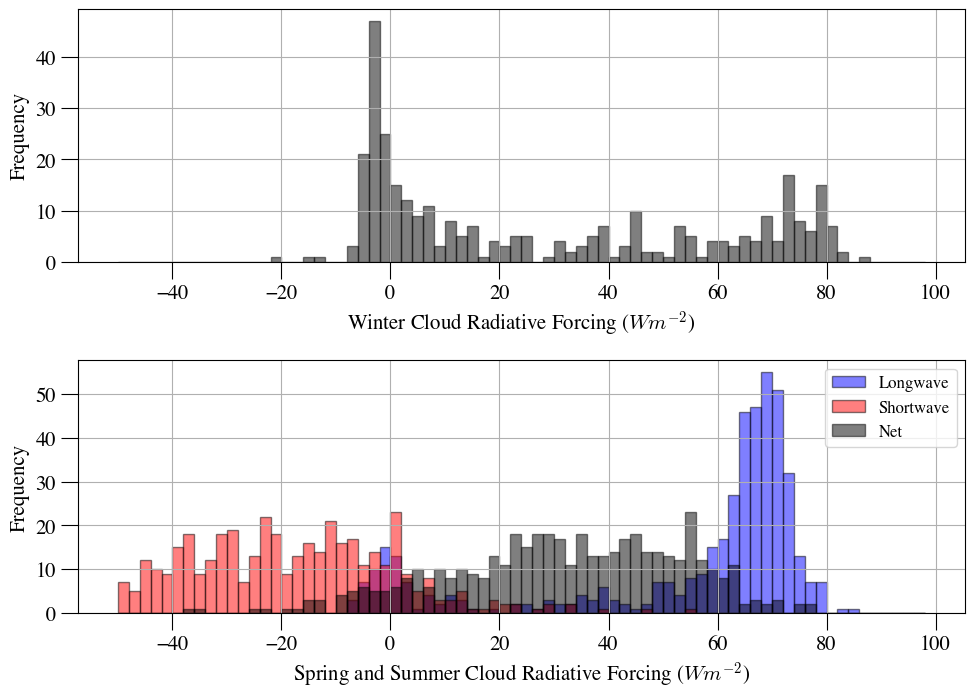
\includegraphics[width=1\linewidth]{figures/chapter4/ForcingValues.png}
    \caption[Histograms of cloud radiative forcing by season.]{Histograms of cloud radiative forcing for winter (top, no shortwave radiation present) and spring/summer (bottom, shortwave radiation indicated in red, longwave in blue, and net in black). For this figure, spring/summer was defined as any time with measurable shortwave radiation.}
    \label{fig:crf_histo}
\end{figure}

Histograms of the longwave, shortwave, and net CRF, shown in Figure \ref{fig:crf_histo}, are divided by season depending on the presence of solar radiation. In winter (top panel), the histogram (LW only) shows a slightly bimodal distribution, with one large peak near 0 $W m^{-2}$ and another small peak between about 50 and 80 $W m^{-2}$. (Note that the negative value of the large peak at 3 $W m^{-2}$ may be due to the slight overestimation in the clear-sky flux as the estimated bias is just under 3 $Wm^{-2}$ for shortwave radiation.) These two modes describe clear (0 $W m^{-2}$) and cloudy (75 $W m^{-2}$) conditions. A range of cloud radiative forcing values is seen leading up to the peak of the distribution at about 85 $W m^{-2}$ due to the range in cloud properties (fraction, phase, height) and their associated radiative impacts during the winter. The winter had quite variable cloud conditions compared to those in summer in terms of height, temperature, and daily fraction. The highest winter CRF occurred during the storm periods when cloud fraction was large, clouds were primarily close to the surface and composed of ice, and the cloud base and surface temperatures both increased.  

In the summer (Figure \ref{fig:crf_histo}, bottom panel), the range of net CRF is smaller relative to winter. This is due to the negative shortwave CRF (cooling) that counteracts some of the positive longwave CRF. Longwave CRF in summer is between about 0 $Wm^{-2}$ and 80 $Wm^{-2}$, with the latter (cloudy) peak being the larger of the two (unlike winter). The majority of clouds during summer result in from 50 to 80 $Wm^{-2}$ of longwave CRF. Shortwave CRF is between about +10 to -30 $Wm^{-2}$, with a few values as low as -50 $Wm^{-2}$. The result of these two competing components of CRF is a slightly bimodal distribution of net CRF, with a small peak near 0 $Wm^{-2}$ and a larger peak between 30 to 70 $Wm^{-2}$. The peak near 0 $Wm^{-2}$ is small due to the limited number of clear-sky days seen during the summer. Clouds were consistently low and thick throughout the spring and summer, resulting in more uniform net CRF values throughout these two seasons than in winter.

\begin{figure}[p]
    \centering
    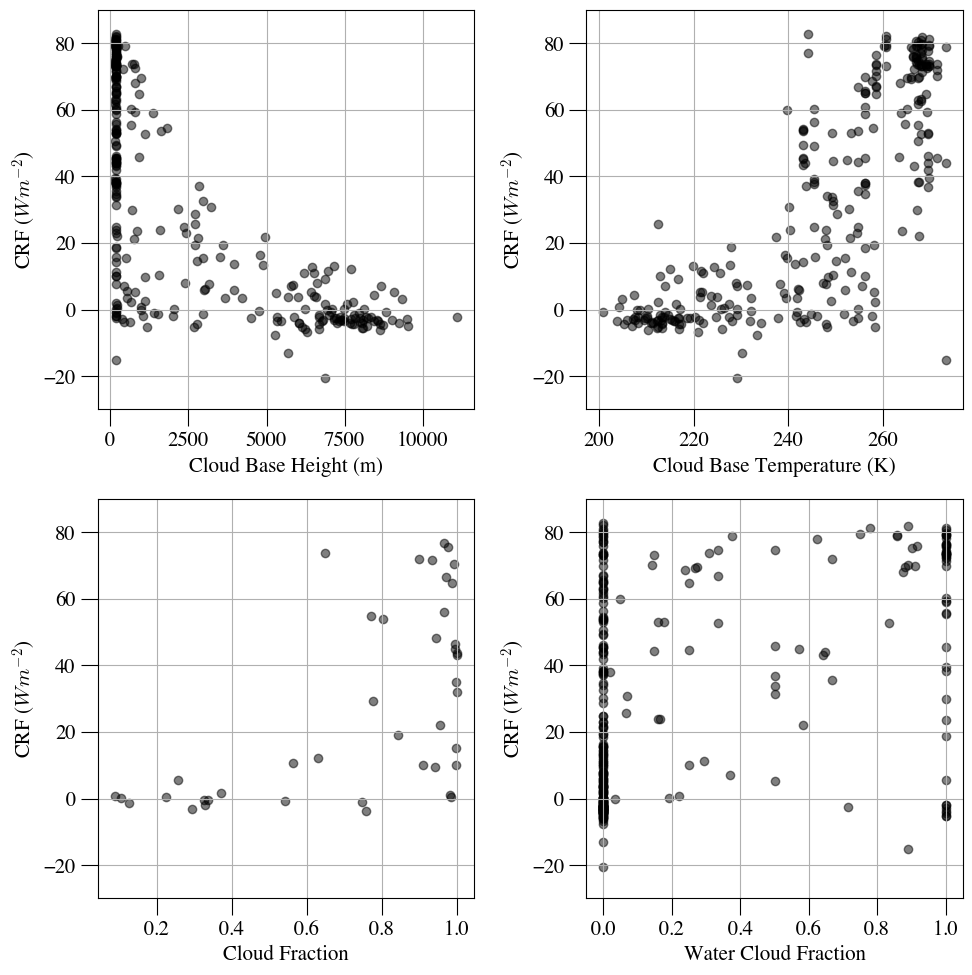
\includegraphics[width=1\linewidth]{figures/chapter4/VSWinter.png}
    \caption[Cloud radiative forcing vs cloud base height, cloud base temperature, cloud fraction, and water cloud fraction for winter.]{Cloud radiative forcing vs cloud base height (top left), cloud base temperature (top right), daily mean cloud fraction (bottom left), and water cloud fraction (bottom right) for the winter season (defined as the period when no shortwave radiation is present). Net cloud radiative forcing is only comprised of longwave radiation during this time of year, so black dots represent both the net longwave CRF and the net CRF.}
    \label{fig:winter:crf}
\end{figure}

\begin{figure}[p]
    \centering
    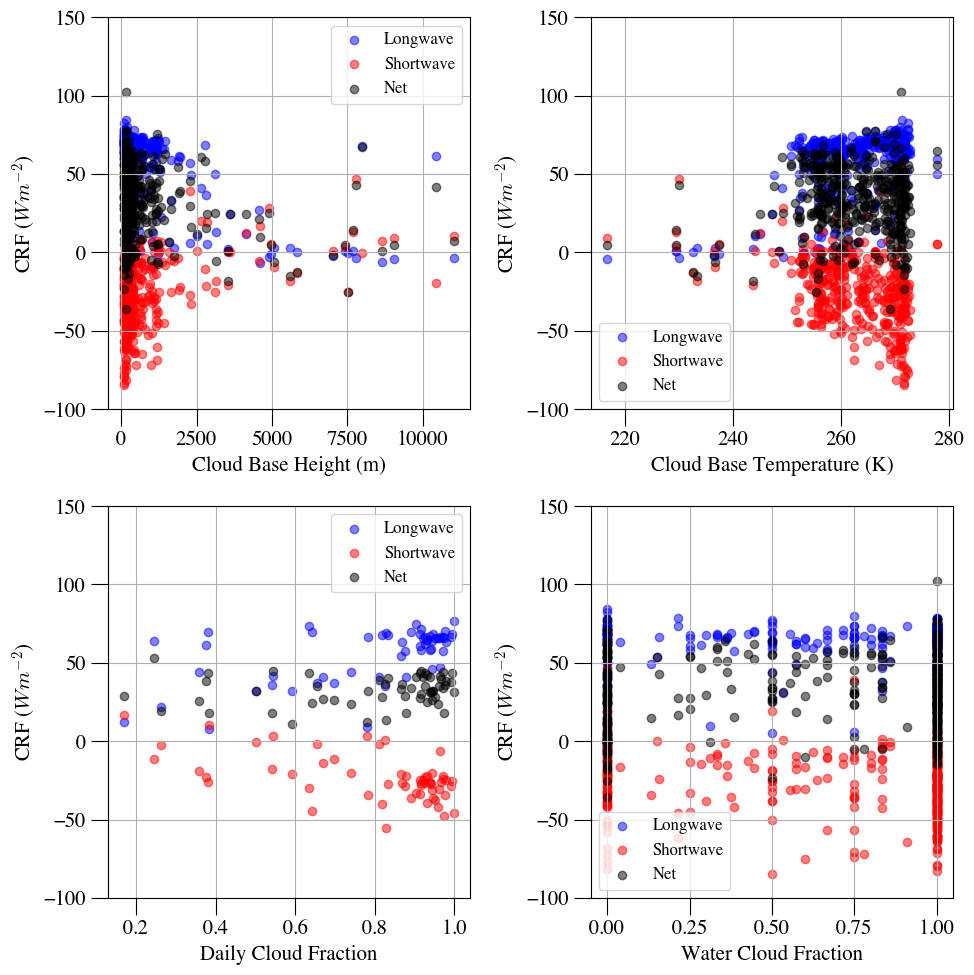
\includegraphics[width=1\linewidth]{figures/chapter4/VSSummer.png}
    \caption[Cloud radiative forcing vs cloud base height, cloud base temperature, cloud fraction, and water cloud fraction for summer.]{Cloud radiative forcing vs cloud base height (top left), cloud base temperature (top right), daily mean cloud fraction (bottom left), and water cloud fraction (bottom right) for the spring/summer season (defined as the period measurable shortwave radiation is present). Longwave radiation is represented by blue dots, shortwave by red dots, and net by black dots in each scatter plot.}
    \label{fig:spring:crf}
\end{figure}

Figures \ref{fig:winter:crf} and \ref{fig:spring:crf} display how the net cloud radiative forcing depends on the cloud's macrophysical properties. Figure \ref{fig:winter:crf} is for winter (Floes 1 and 2), and Figure \ref{fig:spring:crf} is for spring and summer (Floes 3 and 4). During the winter, cloud base height, and cloud base temperature have the most effect on the net CRF. This is no surprise as the free atmosphere is warmer close to the ground, resulting in low clouds having a larger longwave influence on the surface. \citet{shupe:2004} found that clouds with temperatures cooler than 243 $K$ (-30$^{\circ}C$) often had similar longwave radiative properties to clear sky conditions. In winter at N-ICE, there is a transition in radiative values around 235 $K$. Winter clouds with base temperatures greater than 235 K had a larger spread in cloud radiative forcing values of about 60 $Wm^{-2}$. Values lower than this still had variation in CRF, but were within 20 $Wm^{-2}$ of clear-sky conditions and were more sensitive to changes in cloud base temperature. In the summer, this transition occurred closer to the 243 $K$ cutoff reported by \citet{shupe:2004}. However, due to the limited number of high, cold clouds, there were not many clouds below this threshold. In summer the LW CRF was close to zero for these lower temperatures, in better agreement with the results from \citet{shupe:2004}. 

Daily mean cloud fraction (\ref{fig:winter:crf} and \ref{fig:spring:crf}, lower left panels) does not have as clear of a correlation with daily mean surface CRF; days with below 50$\%$ cloud fraction have less than 10 $Wm^{-2}$ of CRF, while days with cloud fraction greater than 50$\%$ can have CRF values that range from around 0 to just under 80 $Wm^{-2}$. These slight trends were also seen by \citet{shupe:2004} during the SHEBA experiment. 

In spring and summer, the relationships between cloud base height and cloud base temperature are less obvious. This is due to the lack of variety in cloud characteristics during this period and the dependence on solar zenith angle. Most clouds were below 2 $km$ with cloud base temperatures above 250 $K$. Periods of higher, cooler clouds were present only during a few storm periods, one near the end of the experiment. These clouds had a higher ice fraction than the other summer clouds, likely due to their height. Cloud properties (such as height, phase, and temperature) have a large influence on longwave radiation.

There is no apparent correlation between the fraction of cloud that is water and the amount of CRF in either season. \citet{schweiger:1999} started that the relationship between particle size and the amount of longwave CRF is not significantly different for liquid and ice particles. They did report a significant difference, however, in shortwave CRF, as the different shapes have different influences on shortwave scattering. However, results from N-ICE do not show differences in water and ice clouds. This is likely due to the inability to determine the thickness of the cloud, as the lidar pulse will attenuate near the base of optically thick clouds, and the wide variety of solar zenith angles that were experienced during the transition to summer. 

The cloud macrophysical and radiative effects seen here could be representative of conditions that are becoming more prominent with climate change. A thorough understanding of the cloud influence on the surface is vital both for forecasting local impacts, such as ice melt or change in surface fluxes, and for use in larger climate circulation models for a more accurate understanding of global climate change. 

\section{Cloud Radiative Forcing modeled by Polar WRF}
Cloud radiative forcing from the Weather Research and Forecasting model (WRF) with polar enhancements (described in Chapter 3) is shown in Figure \ref{fig:wrf_crf_all}. Two model simulations were selected based on their performance in spring and summer during N-ICE. The model run using the Morrison Bulk Two-Moment cloud microphysics (CM) scheme and the Mellor–Yamada Nakanishi Niino (MYNN) planetary boundary layer (PBL) scheme (2-MYNN, purple) had the lowest biases in latent and sensible heat fluxes in the winter. In the spring, the run with the Goddard CM scheme and Mellor–Yamada–Janjic PBL scheme (G-MYJ, orange) had the lowest biases in latent and sensible heat fluxes and net shortwave flux. For more details about the model setup and the strengths/weaknesses of the PBL and CM schemes, see Chapter 3.

\begin{figure}[t]
    \centering
    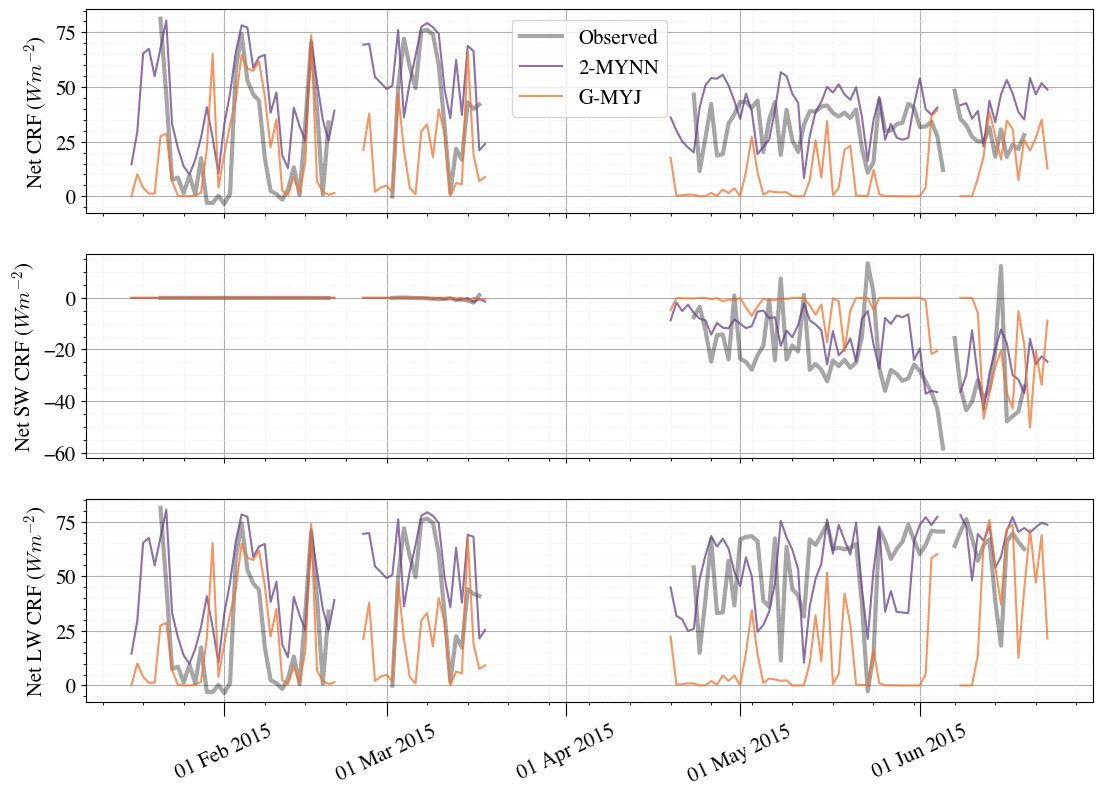
\includegraphics[width=1\linewidth]{figures/chapter4/CRF_TS.png}
    \caption[Time series of cloud radiative forcing in two WRF model runs.]{Net (top), longwave (bottom), and shortwave (middle) CRF from the N-ICE measurements (gray) and modeled by Polar WRF using the Morrison Bulk Two-Moment CM scheme with MYNN PBL scheme (purple) and the Goddard CM scheme with the MYJ PBL scheme (orange).}
    \label{fig:wrf_crf_all}
\end{figure}
\begin{figure}[p!]
    \centering
    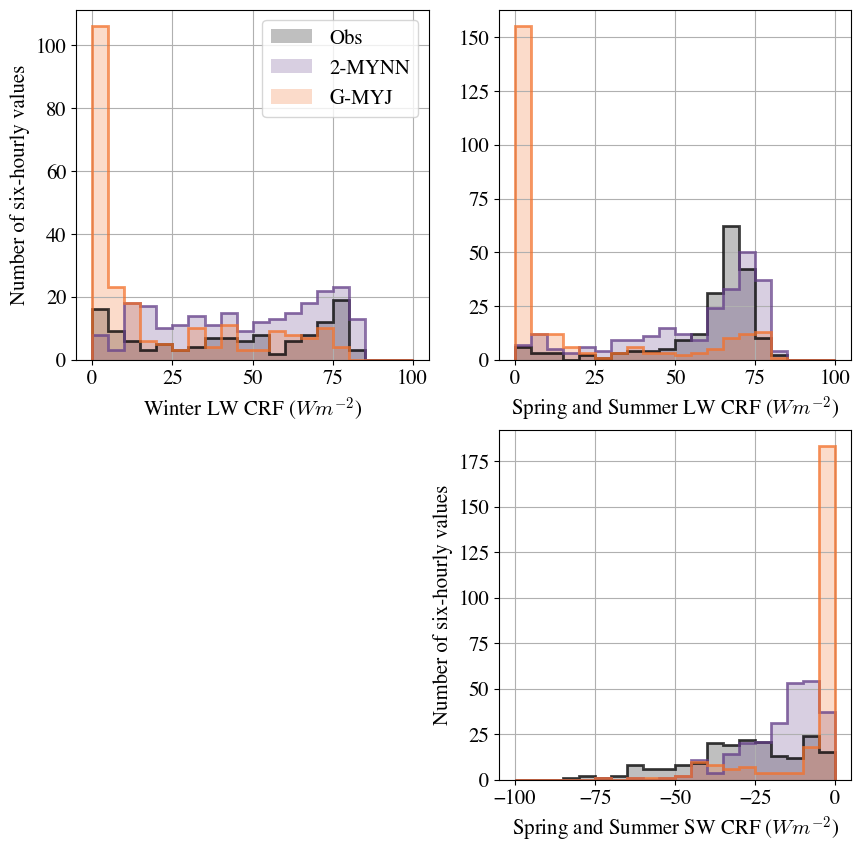
\includegraphics[width=1\linewidth]{figures/chapter4/CRF_Histos.png}
    \caption[Histograms of cloud radiative forcing in two WRF model runs.]{Longwave (top), and shortwave (bottom) CRF in the winter (left) and spring/summer (right). N-ICE measurements  are shown in black. Polar WRF simulated CRF from the Morrison Bulk Two-Moment CM scheme with MYNN PBL scheme (2-MYNN) and the Goddard CM scheme with the MYJ PBL scheme (G-MYJ) are shown in purple and orange.}
    \label{wrf:fig_crf_his}
\end{figure}

The 2-MYNN simulation slightly overestimates CRF throughout much of the N-ICE period. In the winter, CRF is estimated well during times when high CRF values were observed. The model does well with the low, thick clouds that produce high CRF values in the winter. However, in the spring and summer, this scheme underestimates the compensating shortwave CRF, resulting in net CRF values that are too high, regardless of how well the 2-MYNN scheme is reproducing the longwave forcing. The distribution of net longwave forcing can be seen in the top panels of Figure \ref{wrf:fig_crf_his} and the shortwave in the bottom panel.

The 2-MYNN scheme had the lowest longwave bias in the spring. However, the net shortwave bias was the largest with this scheme. Longwave CRF from 2-MYNN did capture some CRF peaks well in the spring, and much of the error in spring CRF is a result of the shortwave CRF. This indicates clouds at N-ICE had a greater influence on the shortwave radiation than those simulated by Polar WRF with the 2-MYNN configuration.

The G-MYJ simulation had the lowest sensible and latent heat flux biases in spring, but greatly underestimates all components of CRF. The G-MYJ simulation displays large net longwave biases. In the spring, the G-MYJ simulation significantly underestimated CRF until the last floe in June. Near the end of June, both model runs began to produce larger CRF values in both the longwave and shortwave. While this increase in longwave and shortwave CRF also increased the net CRF in the 2-MYNN scheme, it balances out to be around 25 $Wm^{-2}$ of net CRF in the G-MYJ scheme, which is similar to CRF values from the N-ICE measurements.

Even the schemes with the lowest biases in the turbulent fluxes simulate large inaccuracies in the modeled CRF. The modeled clouds are not producing the CRF required to replicate the measurements, indicating that the cloud properties are not simulated correctly. This could be caused by some combination of these properities: 1) too few clouds, 2) clouds are not warm enough, or 3) the clouds are not optically thick enough. It is most likely that the cloud fraction is too low because the shortwave flux during the transition from winter to spring is low, especially in the G-MYJ simulation. Figure \ref{fig:wrf_cloudfrac} in Chapter 3 supports this interpretation, showing cloud fraction in the G-MYJ simulation was consistently lower than the measurements, especially in the spring. This figure also shows that the 2-MYNN scheme underestimated cloud fraction throughout the entire spring period.

\section{Conclusions}
The N-ICE field campaign observed unique Arctic atmospheric conditions during the transition from winter to summer over first-year sea ice. As the Arctic continues to move toward ice-free conditions in summer, the need for observations over first-year sea ice becomes increasingly important. There is a need for sufficient measurements to provide valuable comparison datasets for models. Often, models' weaknesses lie in cloud properties. Particularly in the polar regions, where we have fewer observations for validation, the cloud properties are often unknown.

This study aimed to characterize the macrophysical and microphysical properties of the clouds at N-ICE. The cloud phase, base height, and base temperature were explored extensively both for the entire experiment, seasonally, and for a particularly uniquely strong storm-period. 

In the winter, the cloudy and clear conditions described in \citet{graham:2017} were clearly visible in the peaks in the distribution of longwave CRF around 0 $Wm^{-2}$ (clear) and again around 75 $Wm^{-2}$ (cloudy). Spring longwave CRF showed similar results, with an obvious clear and cloudy state. Shortwave CRF in the spring was negative for a lot of the season, with a few positive values as the sun angle continued to become more direct over the field site. Spring and summer were characterized by low, primarily water clouds. Average cloud base height for each month in the spring and summer was below 3 $km$. Winter cloud base heights were higher, particularly those observed in January, when the average cloud base height was over 6 $km$ above the surface.

In winter, the cloud base height and temperature correlated with the CRF. Higher cloud base temperature generally indicated lower CRF values, as the clouds were higher, likely more optically thin, and colder. In the spring, the compensating effects of the LW and SW CRF can be seen. Lower cloud base heights produced increased longwave CRF (as warmer clouds increase LW radiation to the surface), but decreased shortwave CRF (higher clouds are more reflective). The longwave influence dominated the CRF for the entire N-ICE experiment. Had the experiment lasted into mid-summer, it is likely that there would be a short period when the shortwave dominated the CRF as the continued surface melt further lowered albedo, but this period was not reached during the observational period.

Modeled CRF values from the polar WRF model were compared to CRF observations from N-ICE. Longwave CRF was underestimated by the model simulation using the G-MYJ configuration, with the most notable differences occurring during the spring. The G-MYNN run also underestimated SW CRF, resulting in a significant underestimation of net CRF, regardless of this model performing well with latent and sensible heat flux calculations. The 2-MYNN run, the simulation with the lowest wintertime biases in chapter 3, produced LW CRF values similar to those observed at N-ICE. However, the SW CRF was underestimated by this simulation, resulting in a larger net CRF than was observed. In the winter, the 2-MYNN accurately predicts high CRF values but overpredicts low CRF values. In the spring, the opposite is true, higher CRF values are overestimated by the model, but lower CRF value clouds are relatively well modeled.


  \chapter{Latent and Sensible Heat Flux Calculations over First-Year Sea Ice}
\vspace{1 cm}
\begin{spacing}{1} \begin{quote} 
\noindent \emph{A recent review of the latent and sensible heat flux accuracies over the period 2000–2007 highlights significant differences between several gridded products over ocean, where root-mean-squared differences between the multi-product ensemble and data at more than 200  moorings reached up to 25 $W m^{–2}$ for latent heat and 5 $W m^{–2}$ for sensible heat. This uncertainty stems from the retrieval of flux-relevant meteorological variables, as well as from differences in the flux parametrizations.} \end{quote}
\hspace{6 cm} - IPCC Sixth Assessment Report, August 2021  
\end{spacing}
\doublespacing
\section{Introduction}
% why is SEB important
It is important to fully understand the surface energy budget over sea ice because small changes in radiative and/or turbulent fluxes enact feedbacks that can result in significant climate impacts. Reductions in sea ice have been found to amplify the impacts of global warming \citep{wunderling:2020, ipcc_techsum}. Differences in the surface features and atmospheric conditions present challenges for modeling the surface energy and water budgets \citep{wang:2009}. 

\begin{equation}\label{eq:seb}
F_{s} - C = Q_{net} + H_{s} + H_{l}
\end{equation}

% what is the sensible and latent heat flux physically?
The surface energy budget can be seen in \ref{eq:seb}. The net radiative flux, $Q_{net}$, is the combination of the shortwave and longwave radiation (downward - upward), $F_{s}$ is the energy storage, and $C$ is the heat flux from the underlying ocean \citep{walden:2017}. The turbulent fluxes, $H_{s}$ and $H_{l}$, are the sensible and latent heat fluxes and are the focus of this chapter. Physically, the sensible heat flux represents conduction between the atmosphere and the surface that is driven by the temperature gradient near the surface. As defined here, positive sensible heat flux represents energy into the surface, which would occur when the near-surface atmospheric temperature is warmer than the surface. This is often the case during the winter when either near-surface temperature inversions occur or when warm air is advected over the frozen surface. Negative sensible heat flux values represent energy lost by the surface, which occurs when the surface is warmer than the overlying atmosphere. Latent heat flux is the heat associated with a phase change; positive latent heat flux is representative of deposition, condensation, or freezing at the surface, and negative latent heat occurs during sublimation, evaporation, or melting.

% measuring SEB
Some components of the surface energy budget, such as shortwave and longwave radiation, can be measured directly with radiometers. The sensible and latent heat flux, however, is more difficult to measure. A common approach is to use the Eddy Covariance technique. This is explained briefly by \citet{walden:2017}. First, high-frequency covariance measurements are made at different heights above the surface of temperature, wind speed and direction, and water vapor concentration. LiCor's EddyPro 7 \citep{epro} software is then used to process these measurements. The program conducts calibration and filtering on the raw measurements, then calculates the sensible and latent heat fluxes. the covariance measurements were made by a Campbell Scientific CSAT3 sonic anemometer and gas analyzer operated by researchers from the Norwegian Polar Institute. 

% field campaigns measuring the SEB
The Norwegian Young Sea Ice Field Campaign (N-ICE) in 2015 and the Surface Heat Budget of the Arctic Ocean Experiment (SHEBA) in 1998 both deployed eddy covariance (EC) systems, radiometers, and meteorological towers over sea ice in the Arctic ocean. SHEBA took place over older, multi-year sea ice, and the data collected has been processed both using EC theory and using other methods not requiring the EC system. N-ICE took place over young, first-year sea ice. A description of the turbulent fluxes observed by the EC system and the radiation measured by radiometers can be found in \citet{walden:2017}, which describes the observed surface energy budget at N-ICE. 

\section{Calculating Sensible and Latent Heat Flux}
In this section, the measured turbulent fluxes are compared to two methods of calculating sensible and latent heat flux: a bulk flux algorithm based on Monin-Obukhov similarity theory \citep{foken:2008} and the Maximum Entropy Production (MEP) method \citep{zhang:2021, wang:2014, wang:2009}. Both methods estimate flux without covariance measurements and instead utilize values more commonly observed at weather stations. The following subsection will give details about how the stability is used to calculate the stability-dependant scaling parameters required by equations for both the bulk flux algorithm and the MEP method.  

\subsection{Bulk Flux Algorithm}
The bulk flux algorithms are most commonly used for estimating turbulent fluxes \ref{reeves:2021} in models because they are relatively easy to calculate (depend only on meteorological variables) and are computationally efficient. The bulk flux algorithm formulations of sensible and latent heat flux used here are shown in Eq. \ref{eq:hs} and \ref{eq:hl} and are referred to as the "bulk flux algorithm" for the rest of this paper.

\begin{equation}\label{eq:hs}
H_{s} = \rho c_{p} C_{Hz} w [T_{s} - T_{z}]
\end{equation}
\begin{equation}\label{eq:hl}
H_{l} = \rho L_{v} C_{Ez} w [q_{s} - q_{z}] 
\end{equation}

Sensible and latent heat flux depend on measurements of wind speed potential temperature ($\theta_{s}$ and $\theta_{z}$) and specific humidity ($q_{s}$ and $q_{z}$) at the surface and a reference height, (for this case 2 $m$ and 4 $m$). In these equations, $\rho$ is the density of the air, $c_{p}$ the specific heat of air, $L_{v}$ the latent heat of vaporization, and $C_{hz}$ and $C_{Ez}$ are the heat and moisture exchange bulk transfer coefficients \citep{foken:2008, andreas:311}. Eq. \ref{eq:chz} and \ref{eq:cez} are the generally accepted functions for estimating these coefficients. 

\begin{equation}\label{eq:cez}
C_{Ez} = \frac{\kappa C_{D}^{\frac{1}{2}}}{[ln(\frac{z}{z_{0}})-\varphi_{h}]}
\end{equation}
\begin{equation}\label{eq:chz}
C_{hz} =  \kappa^{2} \left[ ln \left( \frac{z}{z_{0}} \right) - \varphi_{m} \right] ^{-1} \left[ ln \left( \frac{z}{z_{0}} \right) - \varphi_{h} \right] ^{-1}
\end{equation}

These equations are functions of $\varphi_{m}$ and $\varphi_{h}$, the scaling parameters, which depend on the surface stability. They also require estimations of the drag coefficient ($C_{D}$) and the roughness length ($z_{0}$).

\subsection{Maximum Entropy Production Method} 
The MEP method was developed to accurately estimate surface fluxes while limiting the number of empirically-derived values and scaling parameters used. This method is based on the principle of maximum entropy and Bayesian probability theory from statistical mechanics \citep{wang:2014}. Equations \ref{eq:mep:hl}, \ref{eq:mep:hs}, and \ref{eq:mep:rn} are the MEP formulations for sensible ($H_{s}$), latent ($H_{l}$), and surface thermal ($Q_{net}$) energy flux, respectively. 

\begin{equation}\label{eq:mep:rn}
\left[ 1 + B(\theta) + \frac{B(\theta_{pc})}{\theta_{pc}} \frac{I_{wsi}}{I_{0}} | H_{s} | ^{-\frac{1}{6}} \right] H_{s} = Q_{net}
\end{equation}
\begin{equation}\label{eq:mep:hl}
H_{l} = B(\theta_{pc}) H_{s}
\end{equation}
\begin{equation}\label{eq:mep:hs}
Q_{net} = Q_{lw} - H_{l} - H_{s}
\end{equation}

Eq. \ref{eq:mep:b} is required by both the sensible and latent heat flux calculations and needs an estimation of the phase change parameter ($\theta_{pc}$, defined in \citep{wang:2011} as Eq. 9). Calculations of sensible and latent heat flux using this method require estimations of the thermal conductivity \citep{wang:2014} of the surface. The thermal inertia parameter of the sea ice ($I_{wsi}$ \ref{eq:iwsi}) used in the MEP equation requires the air density ($\rho$), specific heat ($c_{p}$), and thermal conductivity or the surface ($\lambda$). \citet{merkouriadi:2017} found that the thermal conductivity of snow on sea ice during N-ICE2015 was much lower than those used in many modeling studies, so the thermal inertia parameter needs to be calculated for our location using an appropriate thermal conductivity value. 

\begin{equation}\label{eq:mep:b}
B(\theta_{pc}) = 6 \left( \sqrt{1 + \frac{11}{36} \theta_{pc}} - 1 \right)
\end{equation}
\begin{equation}\label{eq:iwsi}
I_{wsi} = \sqrt{\rho c_{p} \lambda}
\end{equation}
\begin{equation}\label{eq:i0}
I_{0} = \rho c_{p} \sqrt{C_{Ez}\kappa Z} \left( C_{Hz} \frac{\kappa Zg}{\rho c_{p} T_{r}} \right)^{\frac{1}{6}}
\end{equation}

$I_{0}$ can be calculated by \ref{eq:i0}. This value is called "the apparent thermal inertia of air" by \citet{wang:2009}. It depends on the heat and moisture exchange bulk transfer coefficients ($C_{hz}$ and $C_{ez}$), which are defined in the previous section. In this equation, $\kappa$ is the K\'{a}rm\'{a}n constant, $z$ is the measurements height (2 $m$ for this study), $g$ is the gravitational constant, and $T_{r}$ is a reference temperature of 300 $K$. 

This model has been used to calculate fluxes during SHEBA with some degree of accuracy, proving its ability to perform in the polar regions \citep{wang:2014}. Note that the sign convention for the sensible and latent heat fluxes for this formulation is opposite that given in \ref{eq:seb}, however, this is taken into account in all of the analyses performed here.

\subsection{Surface Stability}
Some commonly accepted sets of equations for the empirical scaling equations ($\varphi_{h}$ and $\varphi_{m}$ for $C_{hz}$ and $C_{ez}$) are shown in Table \ref{tab:stability}. These equations use the surface-layer stability parameter (Eq. \ref{eq:zl}) to determine surface stability. These values depend on the Obukhov length ($L$ Eq. \ref{eq:l}). Obukhov length requires estimations of the covariance of the wind velocity and virtual potential temperature ($\overline{w'\theta_{v}'}$), friction velocity ($u_{*}$), and the virtual potential temperature ($\theta_{v}$). 

\begin{equation}\label{eq:zl}
\zeta = \frac{z}{L}
\end{equation}
\begin{equation}\label{eq:l}
L = -\frac{u_{*}^{3}}{\kappa \frac{g}{\theta_{s}} \overline{w'\theta_{v}'}}
\end{equation} 

Positive surface-layer stability parameter numbers indicate stable conditions and negative indicate unstable conditions. Some studies find that using an adjusted von K\'{a}rm\'{a}n constant ($\kappa$) can improve calculations \citep{businger:1971, zilitinkevitsch:1968, dyer:1970}, but changing this variable is outside the scope of this study, so only formulations using $\kappa = 0.4$ to calculate $\zeta$ are included in Table \ref{tab:stability}. 

{
\begin{table*}[p]
\center
\centering
\scriptsize
    \begin{tabular}{| c | c |}
    \hline
        \rowcolor[HTML]{F3F3F3} \textbf{Author} & \textbf{Equations} \\ \hline
        \shortstack{Swainbank \\ \citep{foken:2008}} & \shortstack{$\varphi_{m} = \begin{cases} 0.613(-\zeta)^{-0.2} & \text{    } -0.1 \geq \zeta \geq -2 \\ \end{cases}$ \\ $\varphi_{H} = \begin{cases} 0.226 (-1/L)^{-0.44} & \text{    } -0.1 \geq \zeta \geq -2 \\ \end{cases}$} \\ 
        \hline
        \shortstack{Tschalikov \\ \citep{foken:2008}}  & \shortstack{$\varphi_{m} = \begin{cases} 1 + 7.74\zeta & \text{    } \zeta \geq 0.04 \\ \end{cases}$\\$\varphi_{H} = \begin{cases} 1 + 5.17\zeta & \text{    } \zeta \geq 0.04 \\ \end{cases}$ } \\ 
                \hline
                \shortstack{Zilitinkevich and \\ Tschalikov \\ \citep{zilitinkevitsch:1968}}  & \shortstack{$\varphi_{m} = \begin{cases} 1 + 1.38 \zeta & \text{    } -0.15 < \zeta < 0 \\ 0.42(-\zeta)^{1/3} & \text{    } -1.2 < \zeta < -0.15 \\ 1 + 9.4 \zeta & \text{    } 0 < \zeta \\ \end{cases}$\\$\varphi_{H} = \begin{cases} 1 + 1.31 \zeta & \text{    } -0.15 < \zeta < 0 \\ 0.41(-\zeta)^{-1/3} & \text{    } -1.2 < \zeta < -0.15 \\ 0.95 + 8.9 \zeta & \text{    } 0 < \zeta \\ \end{cases}$ } \\ 
                        \hline
        \shortstack{Businger et al. \\ \citep{businger:1971}}  & \shortstack{$\varphi_{m} \begin{cases} (1 - 19.3 \zeta)^{-1/4} & \text{    } -2 < \zeta < 0 \\ 1 + 6\zeta & \text{    } 0 < \zeta < 1 \\ \end{cases}$\\$\varphi_{H} \begin{cases} 0.95(1 - 11.6 \zeta)^{-1/2} & \text{    } -2 < \zeta < 0 \\ 0.95 + 7.8\zeta & \text{    } 0 < \zeta < 1 \\ \end{cases}$ } \\ 
                \hline
       \shortstack{Dyer \\ \citep{dyer:1974}} & \shortstack{$\varphi_{m} \begin{cases} (1 - 15.2 \zeta)^{-1/2} & \text{    } -1 < \zeta < 0 \\ 1 + 4.8\zeta & \text{    } 0 < \zeta \\  \end{cases}$ } \\ 
               \hline
        \shortstack{Skeib \\ \citep{foken:1990}} & \shortstack{$\varphi_{m} = \begin{cases} 1 & \text{    } -0.0625 < \zeta < 0.125 \\ (\frac{\zeta}{-0.0625})^{-1/4} & \text{    } -2 < \zeta < -0.0625 \\ \frac{\zeta}{0.125} & \text{    } 0.125 < \zeta < 2 \\ \end{cases}$\\$\varphi_{H} = \begin{cases} 1 & \text{    } -0.0625 < \zeta < 0.125 \\ 0.95(\frac{\zeta}{-0.0625})^{-1/2} & \text{    } -2 < \zeta < -0.0625 \\ 0.95(\frac{\zeta}{0.125})^{2} & \text{    } 0.125 < \zeta < 2 \\ \end{cases}$ } \\ 
              \hline
       \shortstack{Gavrilov and \\ Petrov \\ \citep{gavrilov:1981}}  & \shortstack{$\varphi_{m} = \begin{cases} (1-8\zeta)^{-1/3} & \text{    } \zeta < 0\\ 1 + 5 \zeta & \text{    } 0 < \zeta\\ \end{cases}$\\$\varphi_{H} = \begin{cases} 0.65 \left[ (1-35\zeta)^{-1/2} + \frac{0.25}{1+8(\zeta)^{2}} \right] & \text{    } \zeta < 0\\ 0.9 + 6 \zeta & \text{    } 0 < \zeta\\ \end{cases}$ } \\ 
               \hline
        \shortstack{Dyer and \\ Bradley \\ \citep{dyer:1982}}  & \shortstack{$\varphi_{m} = \begin{cases} (1 - 28\zeta)^{-1/4} & \text{    } \zeta < 0 \\ \end{cases}$\\$\varphi_{H} = \begin{cases} (1 - 14\zeta)^{-1/2} & \text{    } \zeta < 0 \\ \end{cases}$ } \\ 
                \hline
        \shortstack{Beljaars and \\ Holtslag \\ \citep{beljaars:1991}}  & \shortstack{$\varphi_{m} = \begin{cases} 1 + \zeta + \frac{2}{3} \zeta (6 - 0.35 \zeta) e^{-0.35} \zeta & \text{    } \zeta < 0 \\ \end{cases}$\\$\varphi_{H} = \begin{cases} 1 + \zeta + (1_+ \frac{2}{3} \zeta)^{1/2} (6 - 0.35 \zeta) e^{-0.35 \zeta} & \text{    } \zeta < 0 \\ \end{cases}$ } \\ 
                \hline
        \shortstack{Handorf et al. \\ \citep{handorf:1999}} & \shortstack{$\varphi_{m} = \begin{cases} 1 + 5 \zeta & \text{    } 0 < \zeta < 0.6 \\ 4 & \text{    } \zeta > 0.6 \\ \end{cases}$\\$\varphi_{H} = \begin{cases} 1 + 5 \zeta & \text{    } 0 < \zeta < 0.6 \\ 4 & \text{    } \zeta > 0.6 \\ \end{cases}$ } \\ 
              \hline
       \shortstack{Andreas et al. \\ \citep{andreas:2009}} & \shortstack{$\varphi_{m} = \begin{cases} BDP(\gamma = 16) & \text{    } \zeta < 0 \\ -5z/L & \text{    } \zeta \geq 0 \\ \end{cases}$ \\ $\varphi_{H} = \begin{cases} \varphi_{m}^{2} & \text{    } \zeta < 0 \\ \varphi_{m} & \text{    } \zeta \geq 0 \\ \end{cases}$ } \\ 
        \hline
    \end{tabular}
    \caption[Scaling parameter equations.]{Scaling parameter equations from Micrometeorology \citep{foken:2008} for the universal functions of momentum and heat. 'BDP' represents the Businger-Dyer-Pandolfo relationship, as seen in Eq. \ref{eq:bdp:H} and \ref{eq:bdp:m}. \citep{foken:2008}.}
    \label{tab:stability}
\end{table*}}

Each of the equations shown in the table have different ranges of stability to which they can be applied. These are formulated empirically, meaning they depend on measurements and are useful only under similar conditions \citep{stull:1988, foken:2008}. These equations were selected as they are those listed by \citet{foken:2008} in the book \textit{Micrometeorology} for use using the von K\'{a}rm\'{a}n constant equal to 0.4. One equation, the \citet{andreas:2010} formulation, was selected despite it being absent from the list in \citet{foken:2008}. Many of these equations, with the exception of \citet{andreas:2010}, were created under conditions observed in mid-latitudes. \citet{andreas:2010}, on the other hand, used results from the SHEBA field experiment to tune the relationships based on the Businger-Dyer-Pandolpho (BDP) relationship (Eq. \ref{eq:bdp:m} and \ref{eq:bdp:H}). This relationship is generally used for neutral and unstable conditions \citep{foken:2008}, so it requires tuning for other locations. Unlike many of the equations in Table \ref{tab:stability}, the BDP relationship requires an extra variable, $\gamma$, which is defined empirically for each location.

\begin{equation}\label{eq:bdp:m}
\varphi_{m}(\zeta) = (1 + \gamma \zeta)^{-1/4}
\end{equation}
\begin{equation}\label{eq:bdp:H}
\varphi_{H} = \begin{cases} 
\varphi_{m} & \text{    } \zeta \geq 0 \\ 
\varphi_{m}^{2} & \text{    } \zeta < 0 \\ 
\end{cases}
\end{equation}

The empirically defined $\gamma$ value seen in equation \ref{eq:bdp:m} has been calculated for N-ICE \citep{paulson:1970, chen:2001}. This value was highly variable, making the selection of one number difficult. The mean $\gamma$ value back-calculated for N-ICE was around -5 with a standard deviation of 41. At SHEBA, a value of 16 was calculated for $\gamma$. Because of the large range of calculated $\gamma$ values at N-ICE, it is difficult to capture the fluxes well by selecting just one value. This relationship is used within the MM5 Similarity Surface-layer scheme in WRF \citep{paulson:1970} and is the underlying equation handling these values in the WRF runs from Chapter 3. 

The polar regions experience stronger surface inversions than in lower-latitude locations, and sometimes the stability seen in these locations is too strongly stable for other empirical stability functions to apply. Or if they do claim to be valid under those conditions, they may have little validation for large Obukhov numbers. Under these strongly stable conditions, some methods of estimating the scaling parameters break down. However, these are still the commonly selected scaling parameters and are applied over stable conditions regardless of their design. This paper will use the equations in \ref{tab:stability} with the bulk flux algorithm and MEP equations to calculate latent and sensible heat flux over first-year sea ice. The best relationship and flux equations for use at N-ICE will be selected. 

\section{Observations}
Observations from the Norwegian Young Sea Ice Field Campaign (N-ICE) were used to calculate heat fluxes. Atmospheric measurements of temperature, wind speed, and atmospheric humidity at N-ICE were measured at 20 $Hz$ at three levels (2 $m$, 4 $m$, and 10 $m$) from a meteorological tower constructed on first-year sea ice \citep{walden:2017}. The pressure was reported at sea level, and for this study was used to calculate the pressure at 2, 4, and 10 $m$ using the barometric equation \citep{lente:2020}. N-ICE took place in the Arctic Ocean north of Svalbard from January to June 2015. More information about this field campaign can be found in Chapter 2.
 
 Moisture was measured and reported as relative humidity and was converted to saturation vapor pressure and specific humidity using the Clausius-Clapeyron equation \citep{iribarne:1981} along with the temperature at the corresponding tower height. The bulk algorithm requires two levels of specific humidity, but the MEP formulation only requires the surface net radiation, making it applicable for experiments that acquired measurements at only a single height. All height levels of relative humidity were converted to specific humidity so each measurement level could be used in the bulk algorithm for comparison. 

\section{Results and Discussion}
\subsection{Stability Coefficients}
The stability at N-ICE was calculated using Eq. \ref{eq:zl}. Covariance measurements were made for the entire time period, so we have measured Obukhov lengths for validation from EddyPro processing. Figure \ref{fig:ol} shows the Obukhov length ($L$) calculated with \ref{eq:l} by EddyPro for the entire N-ICE study period. This initial comparison was done to determine if any sources of error could be attributed to errors in the Obukhov length. The EddyPro estimation of Obukhov length produced slightly more negative (unstable) values than those calculated directly using Eq. \ref{eq:l}. 

\begin{figure}[b!]
    \centering
    \includegraphics[width=1\linewidth]{figures/chapter5/ch3_obukhovlength.png}
    \caption[Obukhov length]{The Obukhov length measured during N-ICE and processed using EddyPro (green) and calculated using Eq. \ref{eq:l} (blue).}
    \label{fig:ol}
\end{figure}

The Obukhov length depends on the friction velocity, and the surface below N-ICE is first-year sea ice, a relatively flat surface with limited sources of mechanical turbulence. Friction velocity is a measure of the amount of wind shear \citep{stull:1988}. The mean friction velocity observed at N-ICE was 0.24 $m~s^{-1}$ with a standard deviation of approximately 0.1 $m~s^{-1}$. Friction velocity values from Eddypro were around 0.2 $m~s^{-1}$, with a maximum of about 1 $m~s^{-1}$. The results from EddyPro appear to represent a surface with more wind sheer than those calculated independently of EddyPro. 

\begin{table*}[t]
\centering
\footnotesize
\doublespacing
{
\begin{tabular}{| c | c | c | c | c | c | c |}
 \hline
\rowcolor[HTML]{F3F3F3} & \multicolumn{4}{c|}{\textbf{Mean Error $\left(W m^{-2}\right)$}} &  & \\
\rowcolor[HTML]{F3F3F3}  & \multicolumn{2}{c|}{\textbf{MEP}} & \multicolumn{2}{c|}{\textbf{Bulk}} & & \\
\rowcolor[HTML]{F3F3F3} \multirow{-3}{*}{\textbf{Author}} & $H_{l}$ & $H_{s}$ & $H_{l}$ & $H_{s}$ & \multirow{-3}{*}{\textbf{N}} & \multirow{-3}{*}{\shortstack{\textbf{Stability} \\ \textbf{Range}}} \\
 \hline
 Swainbank & 2.156 & -3.070  & -0.523 & -9.812 & 50 & $-2 \leq \zeta \leq -0.1$ \\ 
 Tschalikov & -1.054  & -7.556  & 0.559 & -63.357 & 312 & $0.04 \leq \zeta$ \\  
 Zilitinkevich and Tschalikov & 1.266 & -3.246 & -0.240  &  -2.065 & 1499 & $-1.2 < \zeta$ \\
 Businger et al. & 1.260 & -2.798  & -0.191 & 0.580 & 1475 & $-2 \leq \zeta$ \\
 Dyer &  1.468  & -2.327 & -0.325  & 7.871  & 1277 & $-1 \leq \zeta$ \\
 Skeib & 1.273 & -2.480  & -0.179 & 5.676  & 1422 & $-2 \leq \zeta \leq 2$ \\
 Gavrilov and Petrov & -0.294 & 2.307 & 0.111 & -28.549 & 1518 & all $\zeta$ \\
 Dyer and Bradley & 2.003  &  -6.299  & -0.511  & 14.959  & 814 & $0 \leq \zeta$ \\
 Beljaars and Holtslag &  -0.270 & 2.674 & 0.100 & 45.403 & 814 &  $0 \leq \zeta$ \\
 Handorf et al. & -0.274  &  2.508  & 0.133 & -39.040  & 814 & $ 0 \leq \zeta$ \\
 Andreas et al. & 0.617 & 0.882 & -0.175  & 5.071  & 1518 & all $\zeta$ \\
 \hline
\end{tabular}}
\caption[Sensible and latent heat flux mean error for each scaling function relationship.]{Mean error sensible and latent heat flux calculations using each scaling equation listed in Table \ref{tab:stability} for both the MEP equations and the bulk flux algorithm. The number of hourly measurements used and the applicable ranges are shown in the rightmost columns.}
\label{tab:stability_error}
\end{table*}

Table \ref{tab:stability_error} shows the mean error when using the MEP and bulk flux methods to calculate surface fluxes relative to the EddyPro results. Each source in the ``Author'' column corresponds to equations in Table \ref{tab:stability}. Each has a different number of hourly measurements included because each is applicable to specific ranges in stability. For example. Swainbank \citep{foken:2008} is only valid for surface-layer stability parameter values between -0.1 and -2, indicating this is only valid for unstable conditions, which we see rarely in the polar regions. So this formulation uses only a small number of observations for comparison. \citet{andreas:311}, on the other hand, was created using the SHEBA observations and has the largest range of value over which it is valid. The equations created by \citet{andreas:311} had the lowest mean error for the latent heat flux when using the MEP equation, however, its performance calculating the sensible heat flux was comparable to other equations considering the same wide range of stability values. 

Using the bulk flux algorithm resulted in similar errors for latent heat flux regardless of the scaling parameter relationship used with the exception of the Swainbank and Tschalikov \citep{foken:2008} formulations, which had a significantly lower and higher mean error, respectively. While Swainbank \citep{foken:2008} did have the lowest mean error for the latent heat flux and one of the lowest for the sensible heat flux, it was not selected for use because of the low number of stability conditions over which it can be used.  

Due to its wide range of stability values and its improved performance for latent heat flux, the \citet{andreas:2010} formulation was used for the final analysis of both the bulk flux equation and the MEP equation. The MEP equation typically uses the relations developed by \citet{businger:1971}, but for our location, the \citet{andreas:311} formulation performed better when compared to the EddyPro measurements when calculating latent heat flux. Sensible heat flux, on the other hand, was comparable between the \citet{andreas:311} formulation and the \citet{businger:1971} formulation. 

\subsection{Thermal Conductivity}
Thermal conductivity is used in the MEP method to calculate the thermal inertia parameter, as shown in Eq. \ref{eq:iwsi}. Thermal conductivity values at N-ICE were much lower than those commonly used in models \citep{merkouriadi:2017}, so special care was taken to ensure that the thermal conductivity estimate was accurate for our conditions. Using the thermal conductivity values shown in Table \ref{tab:thermal} with Eq. \ref{eq:iwsi}, the thermal inertia parameter was estimated for N-ICE as shown in Table \ref{tab:thermal}. 

\begin{table}[t]
\centering
\footnotesize
\doublespacing
{
\begin{tabular}{| c | c | c |}
 \hline
\rowcolor[HTML]{F3F3F3}  & \textbf{Thermal Conductivity} & \textbf{Thermal Inertia}\\
 \rowcolor[HTML]{F3F3F3}\multirow{-2}{*}{\textbf{Floe}} & $(m^{-1}K^{-1})$ & $(J~m^{-2}Ks^{-0.5})$ \\
  \hline
 1 & 314.264 & 0.183  \\
 2 & 429.650 & 0.246 \\ 
 3 & 280.424 & 0.193 \\
 4 & 1009.816 & 0.311 \\
  \hline
\end{tabular}}
\caption[Thermal conductivity and inertia.]{Thermal conductivity and inertia for each floe during N-ICE. Conductivity values were taken as a mean from \citet{merkouriadi:2017} and inertia parameters were calculated using equation \ref{eq:iwsi}.}
\label{tab:thermal}
\end{table}

\subsection{Bulk Flux Algorithm}
Calculating the fluxes using the bulk flux algorithm resulted in more large positive values than was seen in the EddyPro or in the MEP results. These can be seen in Figure \ref{fig:bulk:sensible}. In spring, the sensible heat flux is consistently over-estimated by the bulk flux algorithm, indicating that the temperature difference between the surface and the atmosphere is too large in the calculations, and too much heat is being transferred into the surface. The latent heat fluxes, shown in Figure \ref{fig:bulk:latent}, were also significantly larger than the EddyPro results when using the bulk flux algorithm. 

\begin{figure}[h!]
    \centering
    \includegraphics[width=1\linewidth]{figures/chapter5/BulkSensible.png}
    \caption[Sensible heat flux from a bulk flux method compared to EddyPro.]{The sensible heat flux at N-ICE as calculated with EddyPro (green) and with the bulk flux algorithm method (blue).}
    \label{fig:bulk:sensible}
\end{figure}
\begin{figure}[h!]
    \centering
    \includegraphics[width=1\linewidth]{figures/chapter5/BulkLatent.png}
    \caption[Latent heat flux from a bulk flux method compared to EddyPro.]{The latent heat flux at N-ICE as calculated with EddyPro (green) and with the bulk flux algorithm method (blue).}
    \label{fig:bulk:latent}
\end{figure}

In June, there was a large decrease in the latent heat flux according to the bulk algorithm. This was mirrored by an increase in the sensible heat flux. However, this decrease (increase) in the latent heat flux (sensible heat flux) was not seen in the EddyPro results. EddyPro produced latent heat flux values consistently around zero during this time period, while the sensible heat flux became negative. This indicates that the near-surface air was cooler than the surface and sensible heat transfer was occurring instead of a phase change. However, the bulk flux algorithm favored a phase change, likely melting, over a sensible heat flux change. At this time in the experiment, there likely was significant phase change occurring as many melt ponds were developing in the surrounding area \citep{walden:2017}. Overall, latent heat flux values estimated by the bulk equation are more largely positive in the winter and more largely negative in the summer, indicating the bulk flux algorithm shows more melting in the spring and more freezing in the winter than the EddyPro results. 

Positive latent heat flux values in the winter represent surface freezing. These values are, at times, almost 10 $Wm^{-2}$ greater in the bulk results than in the EddyPro results. EddyPro, once again, favors sensible heat flux changes to phase changes. However, the sensible heat flux in the bulk algorithm and in EddyPro are comparable. This indicates that EddyPro is not just favoring the heat transfer to be in the form of sensible heat flux, but it also underestimates the latent heat flux in general, even in situations when it cannot be described by an offset in the sensible heat flux. 

 \subsection{Maximum Entropy Method}
Sensible heat flux from the MEP method was calculated using Eq. \ref{eq:mep:hs}. The results of this are shown in Figure \ref{fig:mep:sensible}. For most of the experiment, the MEP method accurately represented the sensible heat fluxes at N-ICE. In the winter, fluxes were slightly underestimated by the MEP equation, resulting in a bi-modal shape to the distribution shown on the right of the figure. In the spring, there was one occurrence lasting several days with largely negative sensible heat flux shown in the EddyPro results while the sensible heat fluxes from the MEP equation were positive. 

\begin{figure}[h!]
    \centering
    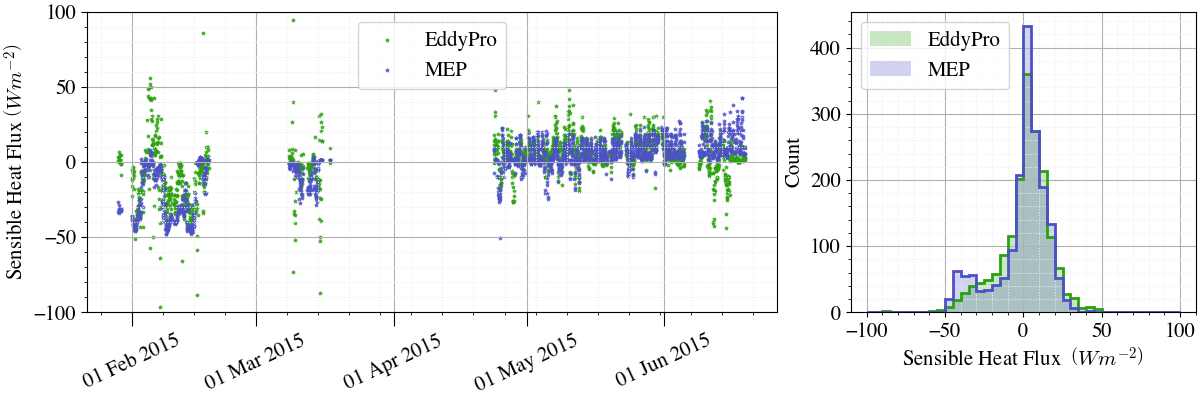
\includegraphics[width=1\linewidth]{figures/chapter5/MEPSensible.png}
    \caption[Sensible heat flux from the MEP method compared to EddyPro.]{The sensible heat flux at N-ICE as calculated with EddyPro (green) and with the MEP method (blue).}
    \label{fig:mep:sensible}
\end{figure}
\begin{figure}[h!]
    \centering
    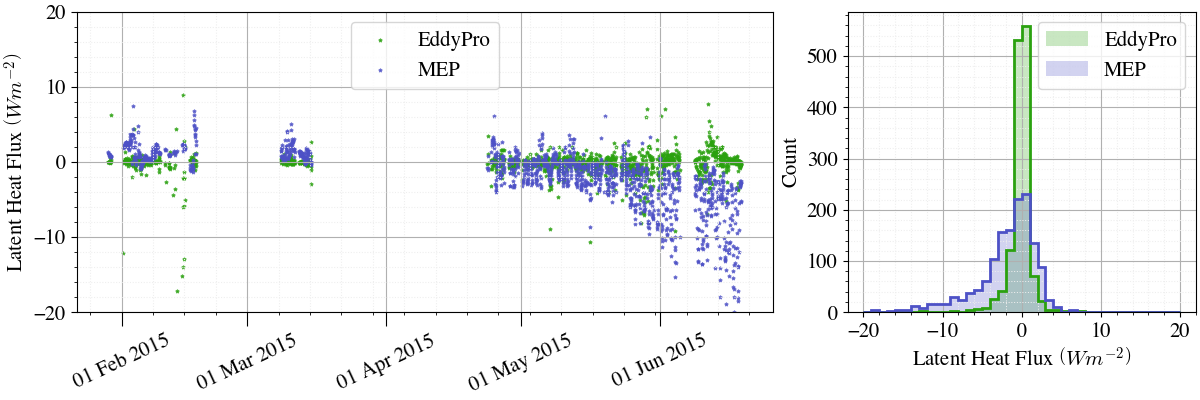
\includegraphics[width=1\linewidth]{figures/chapter5/MEPLatent.png}
    \caption[Latent heat flux from the MEP method compared to EddyPro.]{The latent heat flux at N-ICE as calculated with EddyPro (green) and with the MEP method (blue).}
    \label{fig:mep:latent}
\end{figure}

Latent heat fluxes (Figure \ref{fig:mep:latent}) were not represented as well using the MEP as compared to the EddyPro results. EddyPro showed very small latent heat fluxes throughout the entire experiment. These small heat fluxes were surprising and are not captured with the MEP method. February and March values of latent heat flux are comparable between the MEP and EddyPro calculations, but during spring and entering summer, MEP values are at times 20 $Wm^{-2}$ greater than those calculated by EddyPro, which are rarely greater than 10 $Wm^{-2}$.

\section{Conclusions}
Sensible and latent heat flux formulations require high temporal resolution to use eddy covariance methods. Two methods of calculating sensible and latent heat flux that do not require eddy covariance measurements are explored here. The MEP method is a method utilizing thermal conductivity, net radiative flux, and stability. The bulk flux method requires measurements of moisture and temperature, wind speed, and stability at two levels near the surface. Both equations require the bulk transfer coefficients of heat and moisture, which are a function of stability and have been empirically defined for experiments over a variety of surfaces. Very few of these functions are appropriate for the strong stability conditions that often occur in polar regions. \citet{andreas:311} developed a relationship for these functions that applies to strong stability using data from SHEBA over multi-year sea ice. This relationship was also found to be appropriate for the bulk transfer coefficients at N-ICE using both the bulk flux method and the MEP method. 

The MEP method performed well when compared to the EddyPro values for both sensible and latent heat fluxes. In the winter, the latent heat flux values calculated by the MEP equation are much higher than those in EddyPro, indicating  more phase change. The bulk method also represented the EddyPro values fairly well, although the MEP formulations seem to represent the spread of flux values better than the bulk algorithm. The latent heat flux values were also much larger than those observed during N-ICE in the bulk method. 

Overall, further testing is needed for the validation of the latent heat flux formulations. The latent heat flux values measured at N-ICE were much smaller than expected and smaller than those seen in other experiments, so more measurements are needed to rule out any issue with the N-ICE observations. Both sensible heat flux formulations, however, produced reasonable values over the first-year sea ice seen at N-ICE. 




  \chapter{Improvements to the Weather Research and Forecasting Model over First-Year Sea Ice}

\noindent \textbf{Abstract}

\section{Introduction
}
\section{How does the WRF output (both offline and online) compare with the other formulations (bulk/MEP/EddyPro)?}
\begin{enumerate}
    \item Is MEP a better way to simulate the latent and sensible heat flux over the surface? What if we substituted this into the offline calculation?
\end{enumerate} 

\section{How sensitive is the WRF offline calculation to the universal functions?}

\begin{enumerate}
    \item Can we improve WRF just by implementing a different universal function relationship?
\end{enumerate}

\section{What other things in WRF should be changed to improve performance over first-year sea}
\begin{enumerate}
    \item Cloud properties, surface layer constants, ...
\end{enumerate}

\section{Discussion and Conclusions}



% from my prelim
The global climate is heavily influenced by processes that occur in the Arctic. A lack of observation has led to difficulty understanding atmospheric processes in polar regions \cite{Persson:2002ka}. The IPCC \cite{IPCC:14} lists high to very high confidence in observed changes in marine and terrestrial ecosystems, food production, and health/economics in the polar regions due to climate change. Both the Arctic and Antarctic are projected to continue warming more quickly than the global mean temperature. There is high confidence that year-round sea ice extent has been decreasing since before 1970 and will continue to decrease in the future. The IPCC \cite{IPCC:14} indicates that a changing climate may have large impacts on indigenous people, marine mammals, and coastal ecosystems in the Arctic. However, there are many observational uncertainties, such as in anthropogenic forcings in the polar regions, leading to low confidence \cite{IPCC:14}. Observational uncertainties in these regions stem from the harsh conditions and difficulty in deploying ground-based instruments.

Changes occurring in the Arctic modify the atmospheric circulation, impacting both cloudiness and radiation at the surface \cite{Zhang:2008cn}. According to Stroeve et al. \cite{Stroeve:2012dl}, many CMIP5 members show that there may be ice free conditions within the next couple of years. In addition, Maslanik et al. \cite{Maslanik:2007ha} states that the ice cover can be very sensitive to temperature changes, resulting in large and rapid changes in sea ice extent. Temperatures in the Arctic have increased much more quickly than those elsewhere on the planet, averaging 2 to 3 times faster than the global average, with longer melt seasons and more variability in snow cover \cite{Sledd:2019bz} \cite{AACI:05}. In addition, multi-year ice is disappearing, and being replaced with thin, single-year ice. This movement toward a new ice regime has been referred to as a shift toward a new climate state in the Arctic \cite{Verlinde:2007fu}.  

Arctic amplification is a significant factor in the poles warming more quickly than other parts of the globe. Arctic amplification modifies the surface energy budget. The amplification occurs because of as the Arctic warms, the albedo decreases. The ice-albedo feedback occurs as warmer temperatures cause an increase in ice melt. The albedo of the open ocean or bare land is much lower than that of sea ice or snow, resulting in greater absorption of incoming solar radiation. As the open ocean (or bare surface) absorbs more shortwave radiation, the ocean (land) surface heats, resulting in a greater extent of melt, and therefore further amplification of the ice-albedo feedback. Clouds are an important factor to consider when observing this feedback, as they can enhance or slow surface melt by modifying the energy balance. The presence of clouds can reduce the impacts of sea ice loss by reflecting shortwave radiation away from the earth due to their high albedo, therefore reducing the amount of radiation absorbed by the low albedo surface. Hwang et al. \cite{Hwang:2018jb} states that clouds can reduce the ice-albedo feedback at the surface by around 0.44 Wm$^{-2}$, as was seen in 2007, when a record low sea ice extent was observed \cite{Hwang:2018jb} \cite{Sledd:2019bz}.

The cloud radiation feedback is more dynamic than the ice-albedo feedback in the sense that it can be either positive or negative depending on a variety of influences. Clouds change change the surface temperature by modifying both the shortwave and longwave radiation reaching the surface. Cloud microphysics, such as phase and particle size, as well as macrophysics, including fractional coverage, cloud height and thickness, can influence the amount of radiation reaching the surface and, in turn, influence the impact of the cloud-radiation feedback \cite{Uttal:2002vw}. This relationship is nonlinear and depends on both cloud and sea ice characteristics \cite{Intrieri:2002cn}.

Clouds, as stated above, can modify both the radiation budget and impact the ice-albedo feedbacks. The influence of clouds is magnified by the high surface albedo and the lack of atmospheric moisture \cite{Shupe:2003vt}. Clouds have the greatest potential to modify heat exchange in the Arctic \cite{Intrieri:2002cn}. While we do have some estimates on how much the clouds can impact these feedbacks, more information is needed to quantify the exact influence. Sledd et al. \cite{Sledd:2019bz} states that the clouds are the most important driver in changes in top-of-atmosphere albedo over the entire globe, including at the poles, regardless of the high surface albedo. Cloud characteristics were shown to directly impact the ice thickness in studies by Curry et al. \cite{Curry:1992vn} and Beesley et al. \cite{Beesley:2007vg}.  

The impact of clouds is often quantified using cloud radiative forcing (CRF). The CRF describes how clouds modify the radiation at the surface by taking the difference between the observed radiation and the clear-sky radiation \cite{Ramanathan:1989tl}. When positive radiative forcing is observed, there is a surplus of net radiation at the surface, and warming occurs. When the CRF is negative, cooling occurs at the surface. During clear skies, CRF should equal zero, as the actual radiation should be the same as the estimation of clear-sky radiation. Clear-sky radiation is often calculated from a radiative transfer model or estimated using observed clear-sky times.

Net cloud radiative forcing is a balance of surface warming and cooling due to modifications in radiation as a result of cloud cover. Curry and Ebert \cite{Curry:1992vn} and Intrieri et al. \cite{Intrieri:2002cn} found that, in the Arctic, clouds warm the surface over the entire year (have a positive cloud radiative forcing) except for in mid-July, when the sun highest above the horizon. This nearly year-round warming is due to the small amount of shortwave radiation. When there is solar radiation present, the low sun elevation angle and high surface albedo reflects much of the shortwave radiation away. In addition, the low-level clouds are often emitting longwave radiation at warmer temperatures than the ice surface due to surface temperature inversions \cite{Shupe:2003vt}.

Models in the polar regions have the largest uncertainties relative to other parts of the Earth \cite{Holland:2003hg} \cite{AACI:05}. Models have difficulty simulating radiation accurately during times of thick clouds. A likely reason for this is the model’s inability to estimate the amount of liquid phase drops within the cloud \cite{Graham:2017cs}. A surface inversion often persists over the winter months and processes under these stable conditions are not well understood or modeled \cite{Tastula:2012fta}. In the summer, these inversions are often elevated compared to the wintertime surface inversions \cite{Serreze:1992vz}. Models, however, are integral in understanding the processes occurring in the poles, particularly the radiation.  Unfortunately, few field experiments collecting data for validation exist.

Reanalysis products are often used to study the Arctic climate. This poses a challenge as they are not as thoroughly verified as in other locations due to the extreme climate and dark winters preventing accurate, long-term, multi-season, in-situ and satellite measurements. Biases in clouds result in difficulties in resolving the surface energy budget. Recent studies have shown that when compared with surface observations, reanalysis have large biases in cloud properties (liquid/ice water path, fraction). A number of field experiments have shown that mixed-phase clouds are dominant in autumn through spring in the lower levels at high latitudes \cite{Intrieri:2002cn} \cite{Wang:2005vx}. Cloud micro- and macrophysics are closely tied into the surface energy budget, but parameterizations of such are not well developed in models. Particularly in the Arctic, the radiative properties of clouds and how they are parameterized in models is of importance to modeling the surface energy budget. 

The  Norwegian Young Sea Ice Experiment (N-ICE, described in section 3) field campaign was the first winter field experiment in the Arctic since the Surface Heat Budget of the Arctic (SHEBA) experiment, taking place on-board a research vessel frozen into Arctic sea ice. SHEBA’s primary goals were to observe the surface energy budget, ice mass balance, and ocean-ice-atmosphere interactions in the Arctic during a year-long period from October 1997 to October 1998. Much like N-ICE, SHEBA was motivated by changes in the Arctic and the need for a better understanding of physical processes in the polar regions \cite{Randall:1998up}. A secondary objective of SHEBA was to improve model simulations of the Arctic for use in global climate models \cite{Uttal:2002vw}. Both the ice-albedo feedback and the cloud-radiation feedback were extensively studied using datasets collected during this field experiment. However, this experiment occurred 18 years prior to N-ICE and in a different location of the Arctic, influenced by different synoptic conditions. 

During SHEBA, the Canadian research ship, Des Groseilliers, was allowed to drift with the sea ice. A map of the ship locations in both SHEBA and N-ICE is shown in Figure 1. SHEBA took place across in the Beaufort Sea, with the entire experiment taking place north of Alaska \cite{Uttal:2002vw}. In contrast, the N-ICE campaign took place north of Svalbard. The sea ice during SHEBA was thicker than that during N-ICE, as the experiment was conducted further from the ice edge \cite{Graham:2017cs}. 

During the start of SHEBA, the western Arctic had an anomalously large amount of multi-year ice. In addition, the autumn upper ocean had a lower salinity and warmer temperature than expected, indicating a larger ocean heat flux than was typical of the area during the summer resulting in larger melt due to the reduction in sea ice cover the previous year. Comparing SHEBA data to estimates from other fields experiments showed that during transition seasons (September, October, November, March, and April), SHEBA had larger incoming longwave radiation by 2 to 45 Wm$^{-2}$ than other studies. This could be caused by either an increase in the number of warm air masses over SHEBA or an increase in cloud cover \cite{Persson:2002ka}. SHEBA was an important field experiment that filled many gaps in our understanding of cloud and radiation processes. One of the most important findings from SHEBA was that, even at temperatures well below freezing, mixed-phase clouds occurred often. 
\end{mainchapters}

% Enter the relative directory for your .bib file here
% Default title is ``Bibliography'' and can be
% changed with \makebibliography{bibfile}[New Title]
\makebibliography{\referencedir/references}


% Appendices, remove if not needed
\begin{appendices}
  \chapter{Glossary of Variables and Constants}
\section{Constants and Variables}
\subsection{Alphabetical}

\begin{enumerate}
    \item[]$B(\theta)$
    \item[]$c$, specific heat
    \item[]$C_{Dz}$
    \item[]$C_{Ez}$
    \item[]$C_{Hz}$ 
    \item[]$C_{p}$ specific heat of dry air
    \item[]$CM$ cloud microphysics
    \item[]$CRF$ cloud radiative forcing
    \item[]$F_{d,lw}$, downwelling longwave flux
    \item[]$F_{d,sw}$, downwelling shortwave flux
    \item[]$F_{u,lw}$, upwelling longwave flux
    \item[]$F_{u,sw}$, upwelling shortwave flux
    \item[]$H_{s}$, sensible heat Flux
    \item[]$H_{l}$, latent heat Flux
    \item[]$I_{0}$,
    \item[]$I_{wsi}$, thermal inertia parameter
    \item[]$L$, Obukhov length
    \item[]$L_{v}$, latent heat of vaporization
    \item[]$PBL$ planetary boundary layer
    \item[]$Q$, thermal heat flux
    \item[]$Q_{net, clear-sky}$, net radiative flux under clear-sky conditions
    \item[]$Q_{net, all-sky}$, net radiative flux including cloud influence
    \item[]$Q_{s}$,
    \item[]$Q_{z}$,
    \item[]$q_{*}$, humidity flux scale
    \item[]$T$, temperature
    \item[]$T_{s}$, surface temperature
    \item[]$T_{z}$, air temperature at height $z$
    \item[]$t_{*}$, temperature flux scale
    \item[]$U_{z}$, wind speed at height $z$
    \item[]$U_{*}$, friction velocity
    \item[]$z$, measurement height
    \item[]$z_{r}$,
    \item[]$\frac{z}{L}$, Obukhov stability parameter
\end{enumerate}
\subsection{Greek Letters}
\begin{enumerate}
    \item[$\kappa$] von K\'{a}rm\'{a}n constant
    \item[$\lambda$] thermal conductivity
    \item[$\rho$] air density
    \item[$\varphi_{h}$] heat scaling parameter
    \item[$\varphi_{m}$] moisture scaling parameter
\end{enumerate}

\section{Acronyms}
\begin{enumerate}
    \item[\textbf{2-MYJ}]
    \item[\textbf{2-MYNN}]
    \item[\textbf{5-MYJ}]
    \item[\textbf{5-MYNN}]
    \item[\textbf{ACSE}]
    \item[\textbf{AIDJEX}]
    \item[\textbf{AOE}]
    \item[\textbf{BDP}] Businger-Dyer-Pandolfo relationship
    \item[\textbf{CRF}] Cloud Radiative Forcing
    \item[\textbf{CMIP5}]
    \item[\textbf{ERA Interim}] 
    \item[\textbf{G-MYJ}]
    \item[\textbf{G-MYNN}]
    \item[\textbf{G-YSU}]
    \item[\textbf{IPCC}] Intergovernmental Panel on Climate Change
    \item[\textbf{LSM}] Land Surface Model
    \item[\textbf{MEP}] Maximum Entropy Method
    \item[\textbf{MPL}] Micropulse Lidar
    \item[\textbf{MYJ}]
    \item[\textbf{MYNN}]
    \item[\textbf{N-ICE2015}] The Norwegian Young Sea Ice field Campaign 
    \item[\textbf{P3}] Predicted Particle 
    \item[\textbf{P3-MYJ}] Predicted Particle 
    \item[\textbf{P3-YSU}] Predicted Particle 
    \item[\textbf{PBL}] Planetary boundary layer
    \item[\textbf{PIOMAS}]
    \item[\textbf{SHEBA}] The Surface Heat Budget of the Arctic Ocean
    \item[\textbf{WRF}] Weather Reserach and Forecasting Model
    \item[\textbf{YSU}]
\end{enumerate}
  \chapter{Description of the Norwegian Young Sea Ice Field Campaign}

% this is from my prelim
The Norwegian Young Sea Ice Experiment was conducted during the six-month transition from the winter to summer (January to June) in 2015 in the Arctic ocean north of Svalbard. All instruments were either deployed on-board the Norwegian research vessel \textit{Lance} or on the sea ice nearby the ship. The ship and surrounding camp can be seen in Figure 2.

Measurements of the energy balance and cloud properties (fraction, height, microphysical, and temperature) can give important insight to climate processes and radiative transfer, but are rarely measured together \cite{persson:2002} \cite{schweiger:2004}. The Norwegian Young Sea Ice Experiment (N-ICE2015) is the first experiment to study all of these factors during both winter and summer since SHEBA in 1997 and 1998 \cite{walden:2017}. 

There were several periods of low atmospheric pressure and increased wind speed that were defined as storms. These storms were also accompanied by increases in the integrated water vapor and changes in wind direction \cite{kayser:2017}. Storms are further described in Cohen et al.  \cite{cohen:2017} and Kayser et al. \cite{kayser:2017}. More details about the experiment and datasets collected can be found in Granskog et al. \cite{Granskog:2016dn}. There are three gaps in the dataset resulting from ice breakup. During the experiment, the floe that the ship was anchored to broke apart, resulting in the inability to continue measurements on  the surrounding sea ice. During these times, the instruments were removed from the sea ice, and the ship then sailed to another floe further north on which the instruments were redeployed. Itkin et al. \cite{itkin:2017} describes the proximity to the sea ice edge throughout the experiment. During the majority of the experiment, the ship was stationed between 50 and 250 km from the ice edge. 

A variety of instruments were deployed during the N-ICE campaign that will be used in this project, including  radiosondes, a MicroPulse Lidar (MPL), a meteorological tower, an Eddy Covariance system, and broadband shortwave and longwave radiometers. 

Vaisala RS92-SGP radiosondes were launched from the ice surface (first floe) or the ship deck (following three floes) twice daily around 1100 and 2300 UTC. They recorded temperature, relative humidity, wind speed and direction, pressure, and geopotential height as high as 30 km. Data are recorded by the radiosondes on a two-second time interval and transmitted to the ground using the Vaisala MW31 ground station \cite{kayser:2017} \cite{cohen:2017}. More information and analysis of the radiosondes can be found in Kayser et al. \cite{kayser:2017}.

Data from the MPL were recorded every 14 seconds up to a height of 20 km. The MPL records backscattered light from clouds and operates at 532 nm. The range resolution is 15 m, with a 18 km maximum cloud base height. Signature distance uncertainties are ± 2\% due to timing uncertainties within the instrument. This instrument is more sensitive to water particles than ice, so some cloud types may be biased toward higher percentages of water than ice within the cloud. The MPL is easily attenuation by optically thick clouds. In some instances when a low water cloud is detected, it is possible that more cloud layers exist above this layer that can not be measured by the MPL. 

A meteorological tower was deployed on the ice 300 to 400 m away from the ship. This tower was set up within a few days of anchoring to each new floe and recorded relative humidity and temperature (Vaisala HMP155), pressure (RM Young 61302 V), and wind speed and direction (Lufft Ventus V200A-UMB) at 2 m, 4 m, and 10 m heights. All measurements were collected by a Campbell Scientific CR30000 data logger at 1 second resolution. Periods of missing tower data were reconstructed using temperature and wind information from the ship (sensors mounted 22 to 24 m above the surface). More information about the meteorological measurements, temperature and wind reconstruction using the ship data, a diagram of the meteorological tower set up, and a comparison of the meteorology to SHEBA can be found in Cohen et al. \cite{cohen:2017}.

Radiometers (Kipp and Zonen CMP22 and CGR4) were set up 1 to 1.2m above the surface near the meteorological tower to measure upward and downward components of longwave and shortwave components of radiation. Kipp and Zonen CVF4 ventilation units were used to heat and ventilate the radiometers. More information about the radiometers and an analysis of the surface energy budget can be found in Walden et al. \cite{walden:2017}.

Turbulent flux data was collected by a closed path EC flux system (Campbell CPEC200) at a varying frequency (10 or 20 Hz). This system contains a sonic anemometer and a closed path, infrared gas analyzer. These allow observation of the heat and moment exchanges and the water vapor and carbon dioxide mixing ratios, respectively. This system was set up next to the meteorological tower over a snow covered surface. Further information about the EC Flux system can be found in Walden et al. \cite{walden:2017}.

\section{Atmospheric components of the surface energy budget over young sea ice: Results from the N-ICE2015 campaign, Walden et al. (2017)}

This paper detailed the turbulent and radiative fluxes over the thin sea ice. Surface and atmospheric conditions were also covered. Snow albedo was around 0.85 in the winter and between 0.72 and 0.80 in the spring and summer. Stable stability was found in the winter, followed by unstable in the spring and approximately neutral in the summer (once 0°C skin temperature was reached). Negative average radiative and turbulent heat fluxes occurred in the winter, ranging between 40 to $0 Wm^{-2}$. In the summer, positive values of as high as $60 Wm^{-2}$ were recorded. Winter sensible heat flux ranged from $20$ to $30 Wm^{-2}$ and spring and summer from 0 to $-20 Wm^{-2}$. Positive values indicate flux into the surface.

My contribution to this publication was to fix several problems with the flux dataset collected during the N-ICE campaign and to process the data through the EddyPro software. The most restrictive data problem was the number of data gaps throughout 30-minute data files, which was caused by a programming error in the datalogger. In some cases, the amount of missing data made the file unable to be processed. To fix this, the data were filled by taking the section of data before it (or after, in the case that the missing data was too close to the start of the dataset) and replicating it for the time period with no recorded data. To ensure that this method of data filling was acceptable, data from Barrow, Alaska was used to compare the post-processed data of a complete dataset with the post-processed results from the same dataset after (artificially added) gaps had been filled. Analysis of both the difference in sensible heat fluxes and the turbulent spectra from before and after the data filling were examined and determined the filling method appropriate for the type of gaps in the N-ICE data. 
  \chapter{Additional Polar WRF Validation Statistics}
\begin{table}[h!]
\center
\centering
\footnotesize
\doublespacing
{
\hspace*{-0.25cm}
\begin{tabular}{| l | c | c | c | c | c |}
\hline
\rowcolor[HTML]{F3F3F3} & \multicolumn{5}{ c|}{\textbf{Winter}} \\
\rowcolor[HTML]{F3F3F3} & \textbf{Temperature} & \textbf{Latent Heat} & \textbf{Sensible Heat} & \textbf{Longwave} & \textbf{Shortwave} \\
\hline
\rowcolor[HTML]{F0F8E6}\textbf{G-YSU}		&	0.3, 0.9, 5.6	&	-1, 0, 5.7	&	-23.4, 0, 34	&	2.9, 0.5, 20.6	&		\\
\rowcolor[HTML]{E0EDF4}\textbf{G-MYJ}		&	-0.1, 0.9, 5.6	&	-0.3, 0, 5.1	&	-22.6, 0.2, 31.8	&	4.4, 0.5, 22.2	&		\\
\rowcolor[HTML]{FEEEF5}\textbf{G-MYNN}		&	0.2, 0.9, 5.3	&	-1.3, -0.1, 5.8	&	-21, 0, 32.6	&	5.2, 0.4, 22.4	&		\\
\rowcolor[HTML]{E0EDF4}\textbf{5-MYJ}		&	0.7, 0.9, 5.6	&	-0.8, 0, 5.2	&	-23, 0.1, 33.2	&	3.4, 0.5, 20.9	&		\\
\rowcolor[HTML]{FEEEF5}\textbf{5-MYNN}		&	2, 0.8, 6.2	&	-1.2, -0.1, 6.4	&	-18.5, 0.1, 29.9	&	8.5, 0.3, 25.7	&		\\
\rowcolor[HTML]{F0F8E6}\textbf{P3-YSU}		&	-7.5, 0.7, 11.7	&	-1.1, -0.1, 5.4	&	-25, 0, 36.8	&	-2.5, 0.2, 28	&		\\
\rowcolor[HTML]{E0EDF4}\textbf{P3-MYJ}		&	3.1, 0.9, 6	&	0.4, 0.1, 4.2	&	-17.2, 0, 29.2	&	12.9, 0.6, 23.1	&		\\
\rowcolor[HTML]{E0EDF4}\textbf{2-MYJ}		&	2.3, 0.9, 5.4	&	-0.1, 0, 4.4	&	-18.3, -0.1, 31.8	&	10.2, 0.5, 23	&		\\
\rowcolor[HTML]{FEEEF5}\textbf{2-MYNN}		&	4.5, 0.9, 7.1	&	0, 0, 4.5	&	-17.1, 0, 29	&	12, 0.6, 22.3	&		\\
\hline
\rowcolor[HTML]{F3F3F3} & \multicolumn{5}{c|}{\textbf{Spring}} \\

\hline
\rowcolor[HTML]{F0F8E6}\textbf{G-YSU}		&	-2.6, 0.9, 4.2	&	2.4, -0.2, 7.7	&	2.2, -0.3, 15.4	&	-33, 0.3, 42.2	&	2.2, -0.3, 15.4	\\
\rowcolor[HTML]{E0EDF4}\textbf{G-MYJ}		&	-2.4, 0.9, 4.1	&	2, -0.2, 6.5	&	2, -0.2, 15.3	&	-32, 0.3, 42.2	&	2, -0.2, 15.3	\\
\rowcolor[HTML]{FEEEF5}\textbf{G-MYNN}		&	-1.8, 0.9, 3.7	&	2.7, -0.2, 7	&	4.1, -0.2, 15.4	&	-27.1, 0.2, 37.9	&	4.1, -0.2, 15.4	\\
\rowcolor[HTML]{E0EDF4}\textbf{5-MYJ}		&	-2, 0.9, 3.6	&	2.7, -0.2, 7.5	&	4, -0.3, 16.9	&	-29.2, 0.3, 39.8	&	4, -0.3, 16.9	\\
\rowcolor[HTML]{FEEEF5}\textbf{5-MYNN}		&	-0.7, 0.8, 3.8	&	3.3, -0.2, 7.3	&	6.3, -0.3, 17.4	&	-22, 0.3, 33.5	&	6.3, -0.3, 17.4	\\
\rowcolor[HTML]{F0F8E6}\textbf{P3-YSU}		&	-9.4, 0.8, 12.2	&	3.3, -0.1, 6.2	&	6.1, -0.4, 21.9	&	-32.2, 0.2, 45	&	6.1, -0.4, 21.9	\\
\rowcolor[HTML]{E0EDF4}\textbf{P3-MYJ}		&	-2.4, 0.9, 4.1	&	2, -0.2, 6.5	&	2, -0.2, 15.4	&	-32.1, 0.3, 42.2	&	2, -0.2, 15.4	\\
\rowcolor[HTML]{E0EDF4}\textbf{2-MYJ}		&	-0.1, 0.9, 3.4	&	5, -0.1, 9	&	7.5, -0.2, 18.1	&	-13.7, 0.4, 29.6	&	7.5, -0.2, 18.1	\\
\rowcolor[HTML]{FEEEF5}\textbf{2-MYNN}		&	2.2, 0.8, 4.1	&	6.5, -0.2, 9.2	&	10.3, -0.3, 18.8	&	-3.3, 0.3, 25.4	&	10.3, -0.3, 18.8	\\
\hline
\end{tabular}
\caption{Mean model bias (left), correlation (middle), and root mean square error (right) for temperature ($K$), latent and sensible heat flux ($Wm^{-2}$), and longwave and shortwave radiation ($Wm^{-2}$). Acronyms represent the MP and PBL schemes (defined in table \ref{tab:schemes}). Rows are ordered by MP scheme and colored by PBL scheme.}
\label{tab:wrfstats}
\end{table}}
\end{appendices}

\end{document} 